
%提出するレポートの書式はこのtemplateファイルに沿って作成してください。
%特に表紙・概要の書式は変えないで下さい。

\documentclass[a4j]{jarticle}

\usepackage[dvipdfmx]{graphicx}
%\usepackage{epsbox}
\usepackage{url}
\usepackage{here}
\usepackage{amsmath,amssymb}
\setlength{\headsep}{-5mm}
\setlength{\oddsidemargin}{0mm}
\setlength{\textwidth}{165mm}
\setlength{\textheight}{230mm}
\setlength{\footskip}{20mm}

\title{
\vspace{30mm}
{\bf 高知工科大学様}
\\
\vspace{5mm}
大学掲示板(KUTBBS)\\
\vspace{5mm}
{\bf  外部設計書v2.0}
\vspace{90mm}
}

\author{
\vspace{5mm}
グループ10 \\
\vspace{5mm}
Pathfinder \\
\vspace{5mm}
\vspace{10mm}
}

%date{
%平成30年8月1日
%}

\begin{document}
\maketitle
\tableofcontents
\newpage




\section{システムの利用と業務の流れ}
本システムは、学生が陥りやすいトラブルや、学生自身の学習における課題や悩みを自主的に解決するための掲示板型のウェブアプリケーションである。近年の情報収集におけるツールと言えば、専らスマートフォンを用いた情報検索であるが、それが必ずしも問題を解決するとは限らない。そこで、(本校の)学生同士が問題をネット上でかつ匿名に解決できるようにするために開発するシステムが、本システムである。



本システムを利用する対象は、本校の学生である。また管理者は、本校の事務員を想定している。新規ユーザは、まず事前に配布される仮ID・パスワードを受け取りこれを本システムに入力することで、ログインすることができる。仮ID・パスワードをそのまま使い続けるのはセキュリティ上好ましくないため、初回ログイン後速やかに変更を促す。管理者の登録については親管理者のみが行える仕様になっている(詳細な仕様はサブシステムの項目で述べる)。登録された管理者は、管理するための業務を行えるようになる。


登録を終えたユーザは、本システムを利用することが可能になる。ユーザは、以下のような主な掲示板の機能を利用することができる。
\begin{itemize}
  \item スレッドの作成及び閲覧
  \item スレッドへの書き込み
  \item ブックマーク機能
  \item スレッド検索
  \item 良いレスに対してアクションを返す機能
  \item 不適切なレスやスレッドの通報
\end{itemize}



管理者が行う主な業務としては、仮ID・パスワード発行と、前述したような例にあたる不適切なスレッドやレスの非表示化(実質的には削除処分)である。また、不適切なスレッドやレスを繰り返し行う悪質なユーザに対して警告や、懲罰措置を行うことも想定されている。そのため、管理者は以下のような機能を利用することができる。
なお親管理者については、これらの操作に加えて管理者の登録も可能である。

\begin{itemize}
  \item 仮ID・及びパスワードの発行
  \item スレッドやレスの非表示化
  \item 通報されてきたスレッドやレスの閲覧
  \item ユーザの情報閲覧
  \item 不適切なユーザへの警告・懲罰機能
  \item 管理者の登録(親管理者のみ)
\end{itemize}





以下に本システムの利用の一例とその過程を示しながら、管理者の業務の流れを示す。

\begin{enumerate}
  \item ユーザAは自身が興味のあるスレッドを閲覧し、書き込みを行った。スレッドを閲覧するために必要な情報は、対象のスレッドに書き込まれたレスの情報のみである。書き込みの際に必要となる情報は、自身の書き込み内容である。

  \item  ユーザが書き込みを行った後、再度書き込みを行ったスレッドを閲覧すると、自分の書き込み宛に誹謗中傷をする書き込みがあったため、管理者に通報を行った。通報を行う際に必要な情報は、不適切なレスが行われたスレッドタイトルと書き込み内容、それに通報の理由である。
  \item  管理者は、Webブラウザから管理者ページにログインし、ユーザから通報されてきたレス及びスレッドを確認するページを閲覧する。管理者は、そのページを閲覧し、公序良俗に著しく欠けるタイトルやレスに対して、非表示化処理を行った。
\end{enumerate}

図1は上記の流れを表したものである。


\begin{figure}[H]
\begin{center}
\resizebox{10cm}{!}{\includegraphics{flow.png}}
\caption{上記の業務の流れ}
\label{fig:figuretest}
\end{center}
\end{figure}














\section{システム概要}
本システムは、メインシステムとして下記に示す「ユーザシステム」、「掲示板システム」、「管理者システム」の3つを実装する。
 また、各システムを構成するサブシステムも併せて示す。それぞれのサブシステムに関しては3章にて詳細を述べる。

\subsection{ユーザシステム}
 ユーザシステムでは、ユーザのアカウント登録や、本システムへのログインをすることができる。また、各ユーザが各種設定を変更したり、お知らせを閲覧したり、ブックマークしたスレッドを容易に閲覧することができる。
\\【構築サブシステム】
\\ ブックマークサブシステム、マイページサブシステム、アカウント登録サブシステム
\\ ログインサブシステム、お知らせ表示サブシステム

\subsection{掲示板システム}
 掲示板システムでは、大学の在学生同士の情報共有の場を提供する。見たいスレッドを検索することができ、
 自分が作成したスレッドに対するレスがついたことを通知できる。また、不適切なスレッドまたはレスに対しては管理者に通報ができる。
 信頼性があるレスに対しては、コレクトボタンを押し、情報の信頼性を示すことができる。
\\【構築サブシステム】
\\ 検索サブシステム、掲示板サブシステム
\\ 通報サブシステム、通知サブシステム、コレクトボタンサブシステム

\subsection{管理者システム}
 管理者システムでは、本システムを管理するための管理者のみが使用できるシステムが備わっている。
\\【構築サブシステム】
\\ 子管理者管理サブシステム、お知らせ編集サブシステム、掲示板編集サブシステム
\\ ユーザ管理サブシステム、ユーザ登録サブシステム、管理者ログインサブシステム

\section{サブシステム設計}
2章で述べた3つのシステムを構成するサブシステムの概要と詳細についてユーザ側、管理者側に分けて述べる。

\subsection{サブシステム概要(ユーザ)}
本システムのサブシステムには、下記のサブシステムが存在する。
\begin{enumerate}
\item アカウント登録サブシステム\\
大学から与えられた仮IDと仮パスワードからユーザ専用のIDとパスワードへ変更し、アカウント登録を行う。

\item ログインサブシステム\\
ユーザが設定したIDとパスワードを入力することで自分のアカウントへのログインを行う。

\item お知らせ表示サブシステム\\
管理者からのお知らせを閲覧することができる。

\item 検索サブシステム\\
過去に作成されたスレッドの検索を行うことができる。


\item 掲示板サブシステム\\
ユーザがスレッドの作成・レスの書き込みを行うことができる。


\item 通報サブシステム\\
ユーザが、誹謗中傷や公序良俗に違反していると考えられるスレッドまたはレスを管理者に通知させることができる。


\item ブックマークサブシステム\\
ユーザは頻繁に訪問するスレッドを登録することができる。


\item 通知サブシステム\\
ユーザが作成したスレッドに対して、レスが書き込まれた場合、またはユーザが書き込んだレスに対して返信が書き込まれた場合に、ユーザに通知を送ることができる。


\item コレクトボタンサブシステム\\
ユーザが投稿したレスに対して、投稿した本人以外のユーザがその投稿内容が確からしいと判断したときに、コレクトボタンを押し、コレクト認定をする。コレクト認定された回数が多いほど、そのレスは信頼性が高いと判断できる。


\item マイページサブシステム\\
マイページでは、ユーザが各種設定を行うことができる。また、ユーザに対する通知がマイページに表示される。
\end{enumerate}

\subsection{サブシステム詳細(ユーザ)}
各サブシステムの詳細を以下に示す。
\begin{enumerate}
  \item アカウント登録サブシステム\\
  アカウント登録サブシステムは以下の機能によって構成される。
  \begin{itemize}
    \item 新規登録機能\\
    新規登録時、ID・パスワード入力画面に遷移する。ユーザは大学から配布された仮IDと仮パスワードを入力することで、ID・パスワード変更画面に遷移することができる。その後、ユーザは各自でIDとパスワードを変更し、登録を行うことができる。なお、IDとパスワードを登録しなければ、本システムは利用することができない。
  \end{itemize}

  \item ログインサブシステム\\
  ログインサブシステムは以下の機能によって構成される。
  \begin{itemize}
    \item ユーザ認証機能\\
    本システムを利用するユーザが、本学の在学生であるかの認証を、IDとパスワードを用いて行う。認証に成功したユーザは、本システムの正当なユーザとして本システムを利用することができる。
    \item ログインボーナス機能\\
    ユーザが本システムにログインしたとき、拡張機能と交換できるポイントが付与される。ポイントが付与される頻度は、1日1回である。1回で付与されるポイント数は10ポイントである。
    \item ログアウト機能\\
    ユーザが本システムにログインしている状態であるとき、「ログアウト」ボタンを押すことで本システムからログアウトすることができる。
  \end{itemize}

  \item お知らせ表示サブシステム\\
  お知らせサブシステムは以下の機能によって構成される。
  \begin{itemize}
    \item お知らせ閲覧機能\\
    管理者から通達されたお知らせを閲覧することができる。
  \end{itemize}

  \item 検索サブシステム\\
  検索サブシステムは以下の機能によって構成される。
  \begin{itemize}
    \item 検索機能\\
    所定の検索テキストボックスに任意の文字列を入力し、その文字列に関連したスレッドを一覧で表示することができる。検索方法はand検索、or検索が使用可能である。
    \item カテゴリ選択機能\\
    所定の検索テキストボックスの横に設置されたカテゴリ選択ボタンで特定のカテゴリを選択すると、選択されたカテゴリ内に存在するスレッドの中から検索することができる。
  \end{itemize}

  \item 掲示板サブシステム\\
  掲示板サブシステムは以下の機能によって構成される。
  \begin{itemize}
    \item スレッド作成機能\\
    スレッドタイトルと最初のレスを入力して、新規のスレッドを作成することができる。
    \item レス書き込み機能\\
    既存のスレッド内に、レスを書き込むことができる。このとき、レス番号・ハンドルネーム・日付・レスIDが表示される。レスの書き込み主がハンドルネームを設定している場合、そのハンドルネームが表示される。
  \end{itemize}

  \item 通報サブシステム\\
  通報サブシステムは以下の機能によって構成される。
  \begin{itemize}
    \item スレッド・レス通報機能\\
    ユーザが誹謗中傷や公序良俗に違反するなどの不適切な内容であると判断したスレッドまたはレスを管理者に通報することができる。このとき、通報者は通報理由を明記しなければならない。
  \end{itemize}

  \item ブックマークサブシステム\\
  ブックマークサブシステムは以下の機能によって構成される。
  \begin{itemize}
    \item ブックマーク登録機能\\
    任意のスレッドをブックマークとしてマイページに登録することができる。
    \item ブックマーク解除機能\\
    マイページに存在する任意のブックマークの登録を解除することができる。
  \end{itemize}

  \item 通知サブシステム\\
  通知サブシステムは以下の機能によって構成される。
  \begin{itemize}
    \item 通知機能\\
    ユーザが作成したスレッドに新たな書き込みがあった場合、またはユーザが書き込んだレスに対して返信が書き込まれた場合に、その旨を通知する。
  \end{itemize}

  \item コレクトボタンサブシステム\\
  コレクトボタンサブシステムは以下の機能によって構成される。
  \begin{itemize}
    \item コレクト認定機能\\
    ユーザが特定のレスに対して、その内容が確からしいと判断した場合、コレクトボタンを押してコレクト認定をすることができる。レスの傍らにコレクト認定された回数が表示されるため、コレクト認定は、ユーザがそのレスの内容が確からしいと判断した指標となる。よって、コレクト認定された回数が多いレスは、信憑性のある情報として、ユーザの情報の取捨選択の判断材料となる。なお、1つのレスに対してコレクト認定できる回数は1回のみであり、コレクトボタンを偶数回押すと、コレクト認定を解除することができる。
    \item ポイント獲得機能\\
    ユーザが書き込んだレスに他のユーザからコレクト認定された場合、レスの書き込み主は拡張機能を解放するためのポイントを獲得することができる。拡張機能とは、スレッドでレスを行う際にレスの表示が変化する機能である。
    ポイント獲得の相場は、1回のコレクト認定につき1ポイントである。1つのレスにおいて、1人のユーザからポイント獲得できる回数は1回のみである(2回目以降のコレクト認定はポイント獲得できない)。また、コレクト認定が解除されたとしても獲得済のポイントが減ることはない。
  \end{itemize}

  \item マイページサブシステム\\
  マイページサブシステムは以下の機能によって構成される。
  \begin{itemize}
    \item ユーザ情報設定機能\\
    ユーザのハンドルネームの設定ができる。ハンドルネームが設定されていない場合は、「名無し」と表示される。
    \item ブックマーク閲覧機能\\
    登録したブックマークの一覧を表示することができる。その中から、任意のスレッドに遷移することができる。
    \item 拡張機能\\
    本システムを利用して得られたポイントと引き換えに、拡張機能が使用可能となる。主な拡張機能としては、取り消し線、太文字、赤字、斜体などが存在する。1つの拡張機能につき、600ポイントを引き換えると想定する。拡張機能は、今後の仕様変更で追加する可能性がある。
    \item 通知設定機能\\
    通知機能のON/OFFの設定をすることができる。
  \end{itemize}
\end{enumerate}



\subsection{サブシステム概要(管理者)}
 管理者ページのサブシステムには下記のサブシステムが存在する。
\begin{enumerate}
  \item 子管理者管理サブシステム\\
  親管理者が子管理者のアカウントを管理するシステムである。親管理者がIDとパスワードを発行することで、本システムを管理する子管理者を登録する。また、不要になった子管理者のアカウントを抹消する。


  \item お知らせ編集サブシステム\\
  管理者からユーザ全体に対して任意のお知らせを通達することができる。


  \item 掲示板編集サブシステム\\
  管理者は不適切であると判断したスレッドやレスを非表示化または置換することができる。


  \item ユーザ管理サブシステム\\
  管理者はユーザの情報を検索し、閲覧することができる。また、不適切なスレッドやレスを書き込んだユーザに対して警告やアカウント凍結などの処置を行うことができる。


  \item ユーザ登録サブシステム\\
  管理者はユーザの仮IDと仮パスワードの発行を行うことができる。仮IDと仮パスワードを用いて、ユーザは本システムに新規登録することができる。


  \item 管理者ログインサブシステム\\
  管理者は学内LANに接続された電子デバイスからのみ、管理者のIDとパスワードを入力することで、管理者として本システムにログインすることができる。
\end{enumerate}

\subsection{サブシステム詳細(管理者)}
各サブシステムの詳細を以下に示す。
\begin{enumerate}

  \item 子管理者管理サブシステム\\
  子管理者管理サブシステムは以下の機能によって構成される。
  \begin{itemize}
    \item 子管理者用ID・パスワード発行機能\\
    親管理者は手動で子管理者用のIDとパスワードを登録し、発行することができる。ただし、子管理者にはこの機能は存在しない。
    \item 子管理者アカウント抹消機能\\
    親管理者は手動で不要になった子管理者のアカウントを抹消することができる。
    \item 子管理者情報閲覧機能\\
    親管理者は子管理者のIDとパスワードを閲覧することができる。
  \end{itemize}


  \item お知らせ編集サブシステム\\
  お知らせ編集サブシステムは以下の機能によって構成される。
  \begin{itemize}
    \item お知らせ編集機能\\
    管理者は、ユーザに対して通達するお知らせタイトルとその内容を編集することができる。
    \item お知らせ表示機能\\
    本システムのトップページに、お知らせ編集機能で編集したお知らせの日付とお知らせタイトルを表示することができる。
    \item お知らせリンク機能\\
    お知らせ編集機能で編集したお知らせ内容を本システムトップページに表示されているお知らせタイトルにリンクを追加することができる。\\
  \end{itemize}


  \item 掲示板編集サブシステム\\
   掲示板編集サブシステムは以下の機能によって構成される。
  \begin{itemize}
    \item スレッド非表示化機能\\
    管理者は、データベースに存在するスレッド及びスレッドに格納された全てのレスを非表示化することができる。
    \item レス非表示化機能\\
    管理者は、データベースに存在するスレッド内のレスを非表示化することができる。
    \item 非表示化履歴閲覧機能\\
    管理者は、非表示化したスレッドまたはレスを一覧で閲覧することができる。
    \item 不適切な単語登録機能\\
    管理者は、誹謗中傷や公序良俗に違反していると考えられる単語を登録することができる。
    \item 不適切な単語自動置換機能\\
    管理者が設定した不適切な単語を検出し次第、自動で伏せ字に置換することができる。
    \item 通報内容閲覧機能\\
    ユーザによって通報されたスレッドまたはレスの内容の一覧を、通報理由と共に閲覧することができる。このとき、通報者のユーザ情報、通報されたスレッド主またはレスの書き込み主のユーザ情報も同時に表示される。\\
  \end{itemize}


  \item ユーザ管理サブシステム\\
   ユーザ管理サブシステムは以下の機能によって構成される。
  \begin{itemize}
    \item ユーザ情報閲覧機能\\
    管理者は、データベースに登録されている任意のユーザ情報を閲覧することができる。
    \item ユーザ情報検索機能\\
    管理者は、データベースに登録されているユーザ情報の中から特定のユーザ情報を検索することができる。
    \item ユーザに対する警告通知送信機能\\
    管理者は、不適切な内容のスレッド作成またはレスの書き込みを度々行ったユーザに対して、注意喚起の旨をユーザのマイページに通知することができる。
    \item ユーザアカウント凍結機能\\
    管理者は、度重なる注意を通達したにも関わらず、迷惑行為が改善されないユーザのアカウントに対して、書き込み不可能にすることができる。\\
  \end{itemize}


  \item ユーザ登録サブシステム\\
   ユーザ登録サブシステムは以下の機能によって構成される。
  \begin{itemize}
    \item 仮ID・仮パスワード発行機能\\
    管理者は仮IDと仮パスワードを発行することができる。仮IDと仮パスワードの生成には、乱数を用いる。\\
  \end{itemize}


  \item 管理者ログインサブシステム\\
   管理者ログインサブシステムは以下の機能によって構成される。
  \begin{itemize}
    \item 管理者認証機能\\
    本システムの管理作業を行うユーザが、管理者であるかの認証を、IDとパスワードを用いて行う。認証に成功したユーザは管理者として本システムの管理を行うことができる。
  \end{itemize}

\end{enumerate}



\section{ユーザインタフェース設計}
%(脚注:レイアウト図の画像は編集途中で、対応する番号や修正などが適応されていない状態です。v2では修正後の画像を表示します。)

本システムが提供する学生掲示板KUTBBSにおける掲示板画面遷移及び各画面の詳細について説明する。

また、本システムが提供する管理者が操作する管理画面における画面遷移及び各画面の詳細について説明する。

\subsection{画面遷移図}
付録\ref{Screen_transition}にて画面遷移図を記載している。
%図\ref{fig:Screen_transition}に画面遷移図を示す。
%\begin{figure}[H]
%\centering
%\resizebox{14cm}{!}{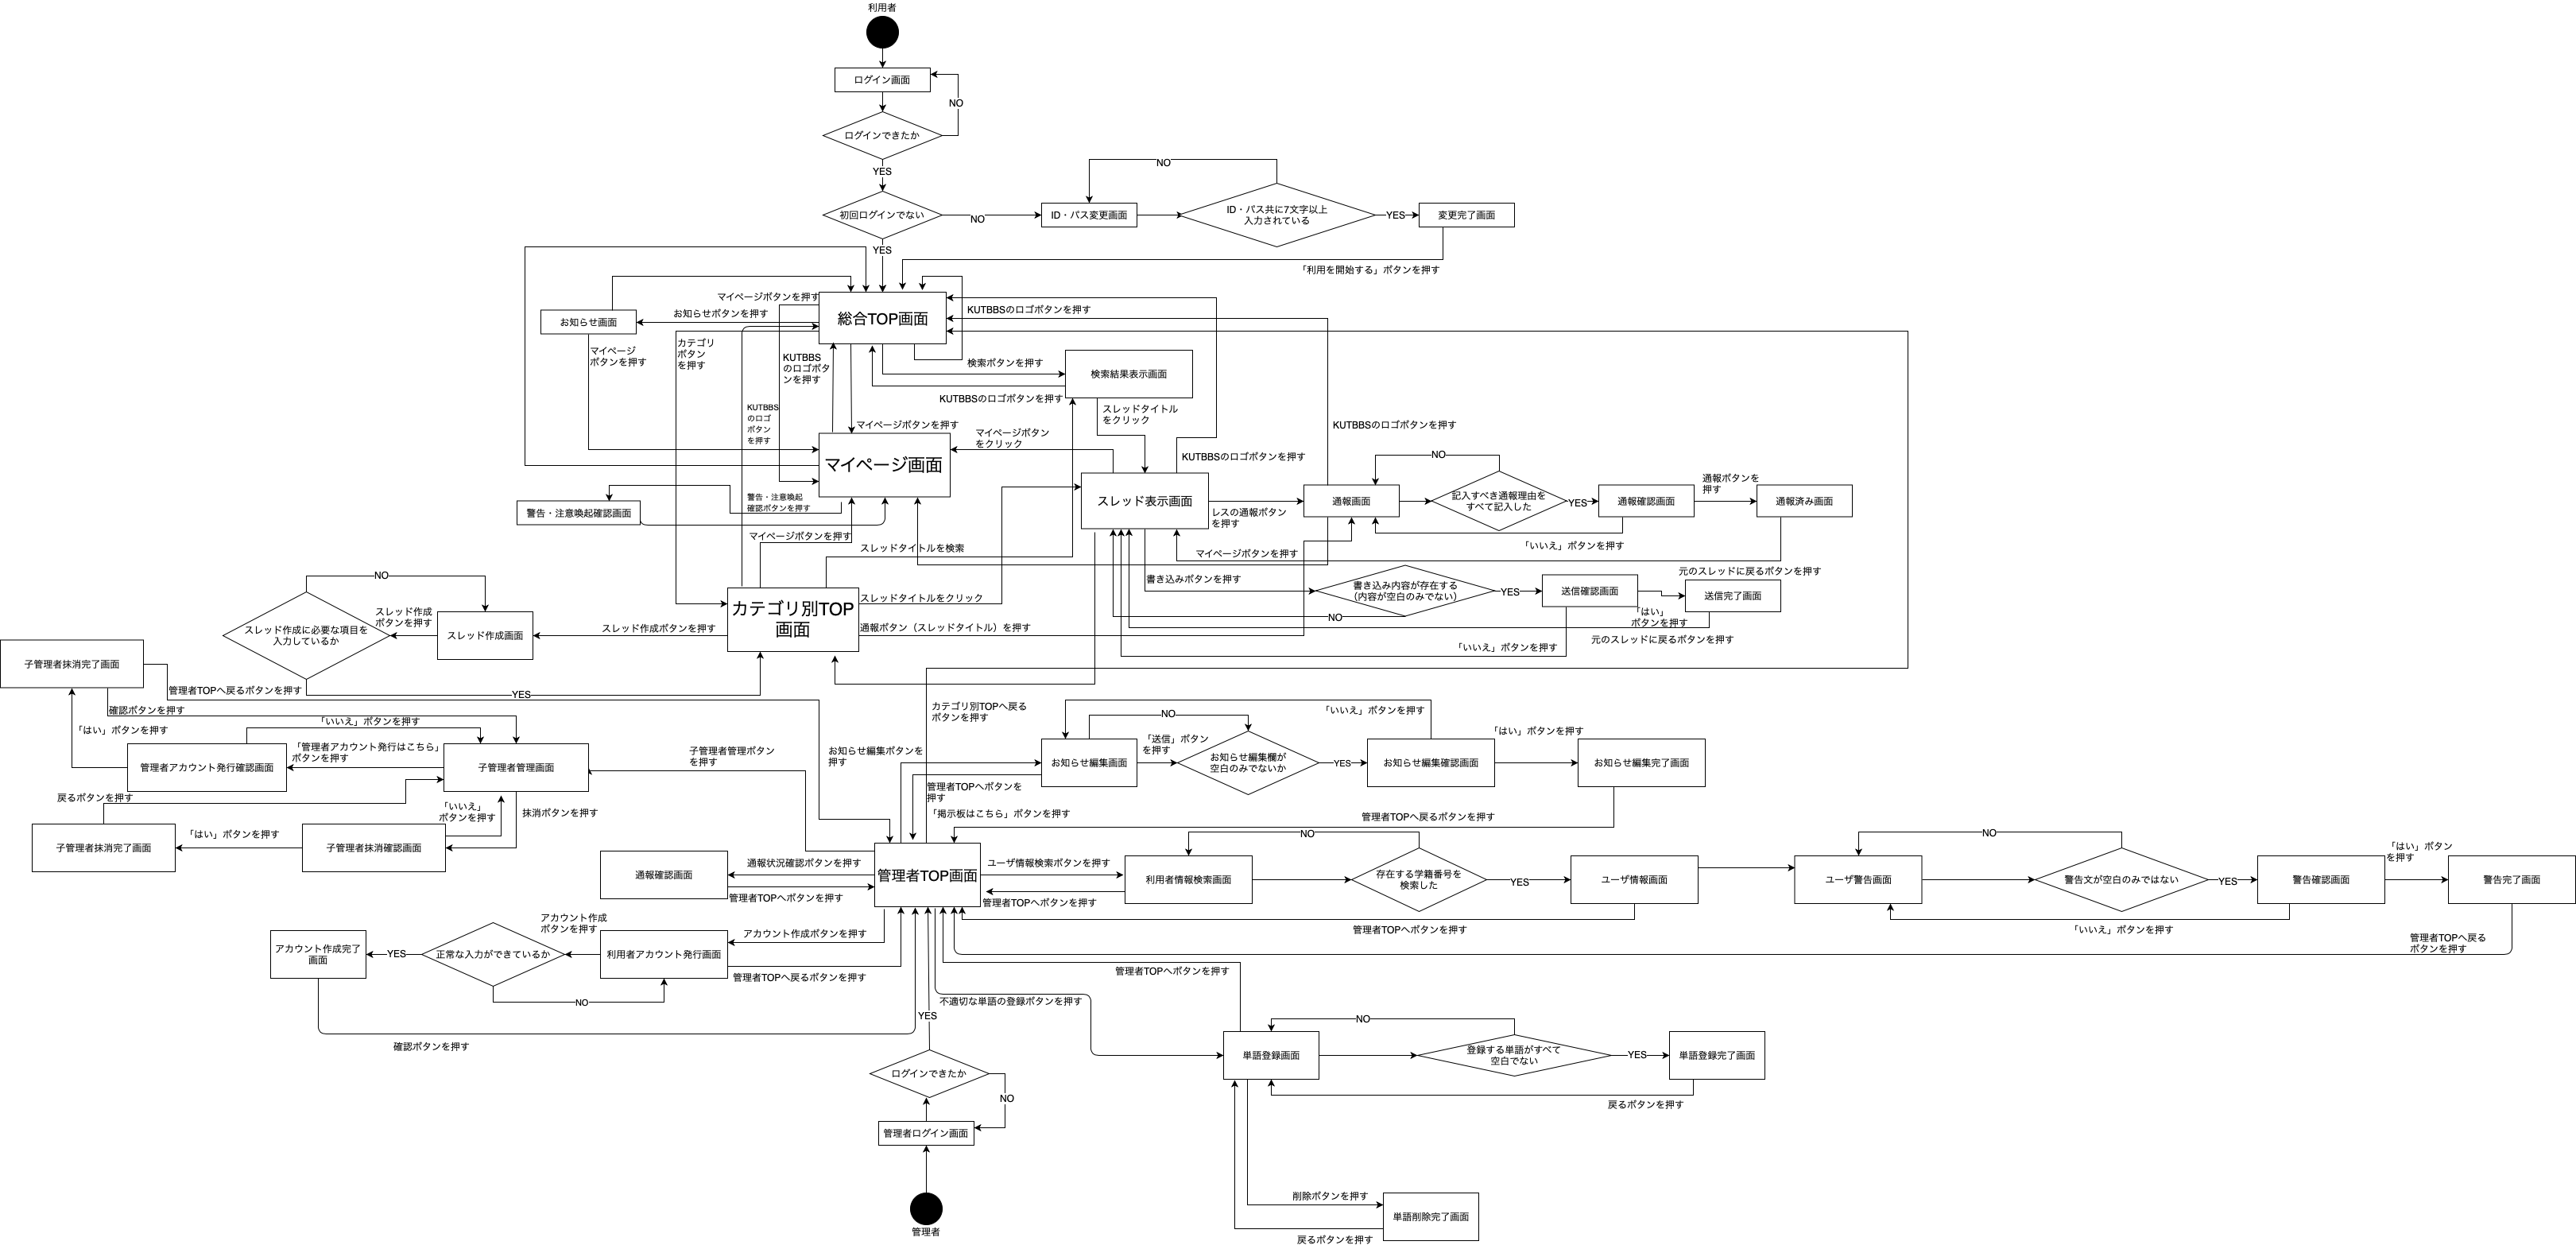
\includegraphics{KUTBBSの画面遷移図.png}}
%\caption{KUTBBSの画面遷移図}
%\label{fig:Screen_transition}
%\end{figure}

\subsection{画面詳細(学生掲示板KUTBBS)}
学生掲示板KUTBBSの画面詳細について記す。各図に示す番号と対応させる形式で、画面内のボタン等の持つ詳細な役割を示す。

また、一部の掲示板の機能はユーザ・管理者ともに使用できるものと管理者のみが使用できるものがあるが、ここでは管理者側で表示する画面を図として用いる。


\subsubsection{ログインTOP画面}
図\ref{fig:login_top}にログインのトップ画面を示す。
\begin{figure}[H]
\centering
\resizebox{14cm}{!}{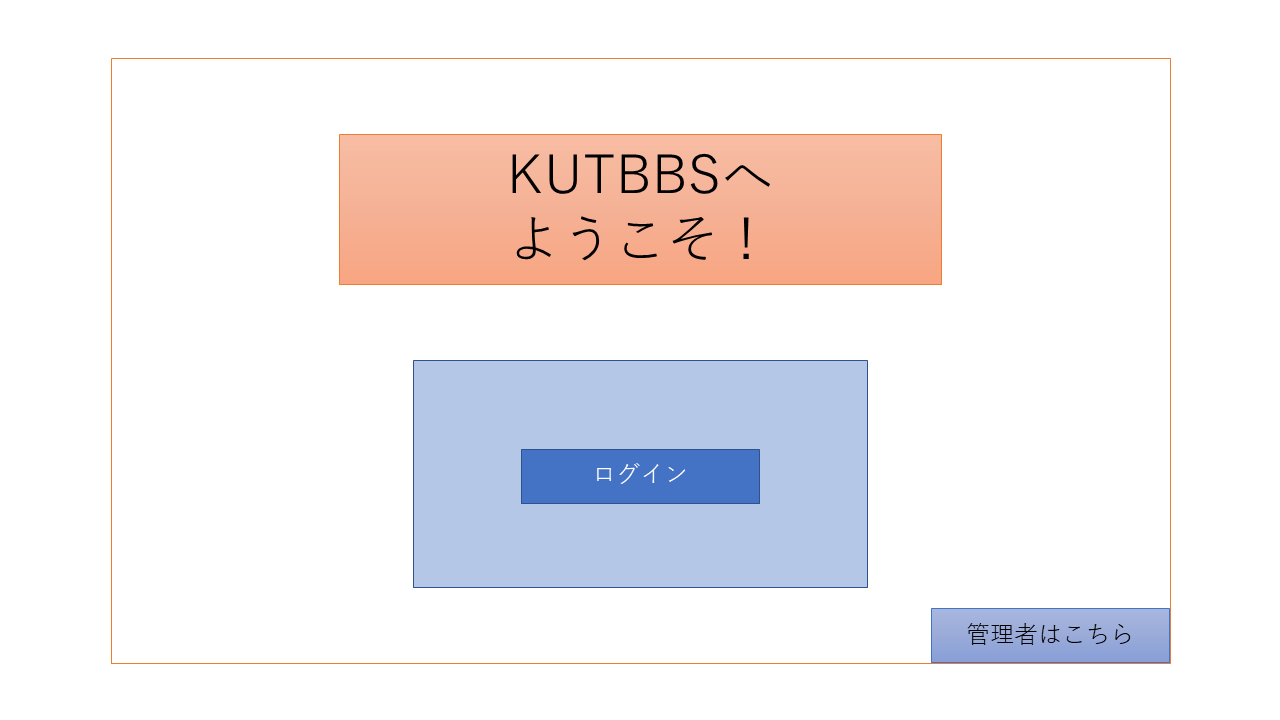
\includegraphics{layout/login_top.PNG}}
\caption{ログインTOP画面}
\label{fig:login_top}
\end{figure}
\begin{enumerate}
  \renewcommand{\labelenumi}{\textcircled{\scriptsize \theenumi}}

\item ログインボタン\\
ユーザはこのボタンを押すことで、図\ref{fig:login_user}に示すユーザログイン画面に遷移する。
\item 管理者はこちらボタン\\
管理者はこのボタンを押すことで、図\ref{fig:login_admin}に示す管理者ログイン画面に遷移する。
\end{enumerate}

\subsubsection{ユーザログイン画面}
図\ref{fig:login_user}にユーザ側のログイン画面を示す。ユーザは自分の持つIDとパスワードを入力する。新規登録ユーザは大学から与えられた仮IDと仮パスワードを入力する。
\begin{figure}[H]
\centering
\resizebox{14cm}{!}{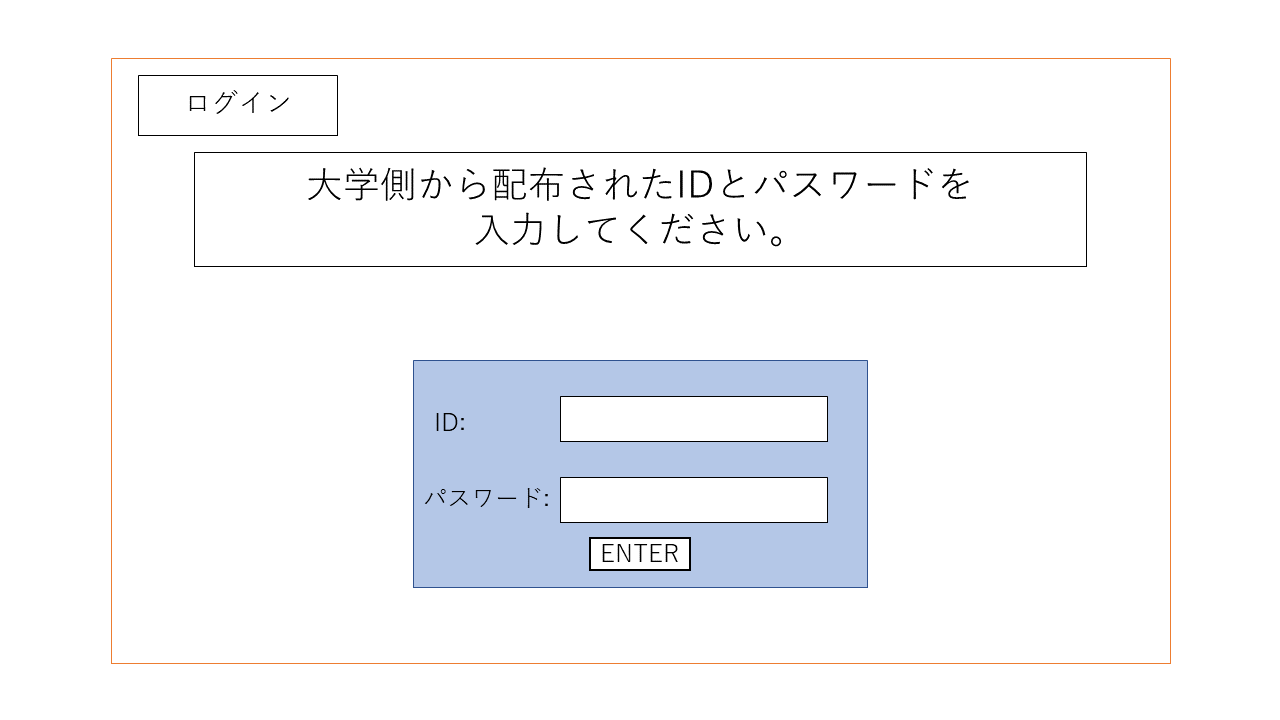
\includegraphics{layout/login_user.PNG}}
\caption{ユーザログイン画面}
\label{fig:login_user}
\end{figure}
\begin{enumerate}
  \renewcommand{\labelenumi}{\textcircled{\scriptsize \theenumi}}

\item ID入力テキストボックス\\
データベースに登録されているIDをテキストボックス内に入力する。
\item パスワード入力テキストボックス\\
データベースに登録されているIDと対応したパスワードをテキストボックス内に入力する。
\item ENTERボタン\\
入力完了時に押すボタンである。テキストボックスに入力されたIDとパスワードがデータベースに登録されている場合、ENTERボタンを押すことで掲示板の総合TOP画面へと遷移する。ただし初回ログインユーザに限り、図\ref{fig:subscribe_user}に示す新規登録画面へと遷移する。入力していない欄がある場合や、入力した内容が一致しなかった場合、エラーメッセージが表示される。
\end{enumerate}

\subsubsection{新規登録画面}
図\ref{fig:subscribe_user}に新規登録画面を示す。ユーザはここで自分が覚えやすいIDとパスワードに変更する。
\begin{figure}[H]
\centering
\resizebox{14cm}{!}{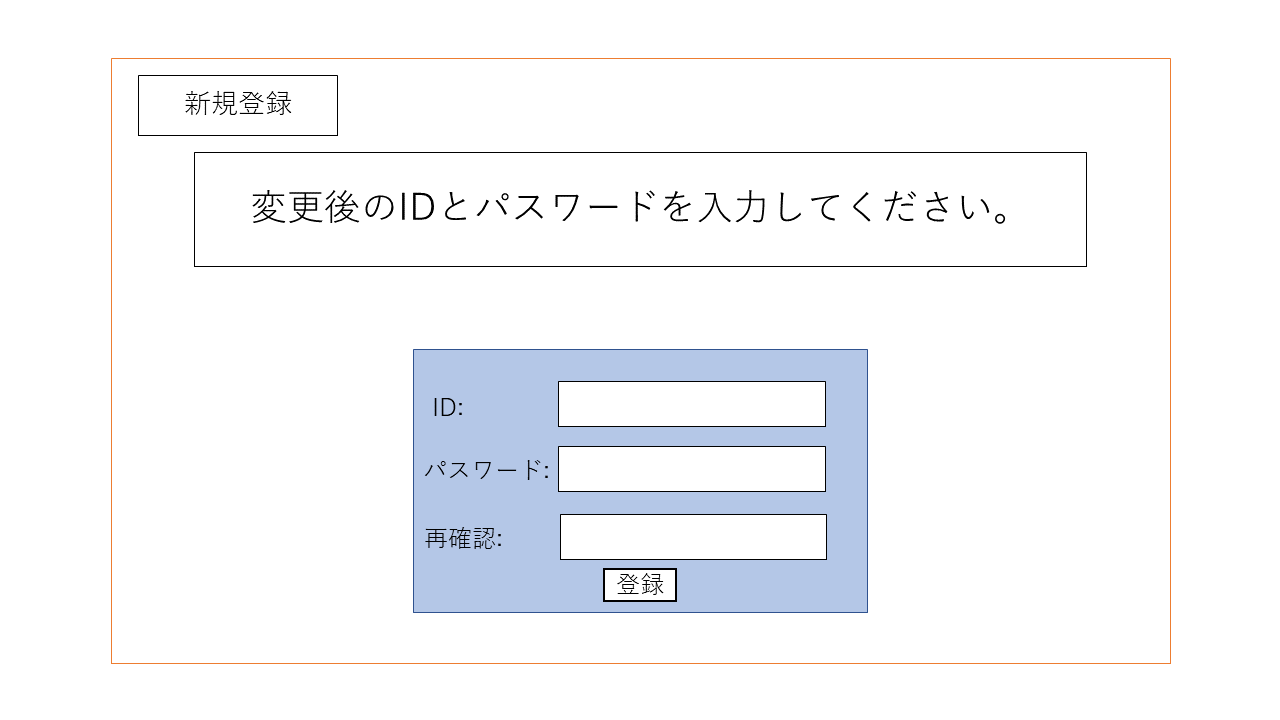
\includegraphics{layout/subscribe_user.PNG}}
\caption{新規登録画面}
\label{fig:subscribe_user}
\end{figure}
\begin{enumerate}
  \renewcommand{\labelenumi}{\textcircled{\scriptsize \theenumi}}

\item ID入力テキストボックス\\
変更後のIDをテキストボックス内に入力する。
\item パスワード入力テキストボックス\\
変更後のパスワードをテキストボックス内に入力する。
\item パスワード再確認入力テキストボックス\\
入力したパスワードを再度入力する。
\item 登録ボタン\\
入力完了時に押すボタンである。テキストボックスに入力されたIDとパスワードがデータベースに登録されている場合、登録ボタンを押すことで掲示板の総合TOP画面へと遷移する。ただし初回ログインユーザに限り、図\ref{fig:BBS_top}に示す新規登録画面へと遷移する。入力していない欄がある場合や、入力した内容が一致しなかった場合、エラーメッセージが表示される。

\end{enumerate}

\subsubsection{新規登録確認画面}
新規登録画面で入力が完了すると、図\ref{fig:subscribe_ok}の新規登録確認画面に遷移する。
\begin{figure}[H]
\centering
\resizebox{14cm}{!}{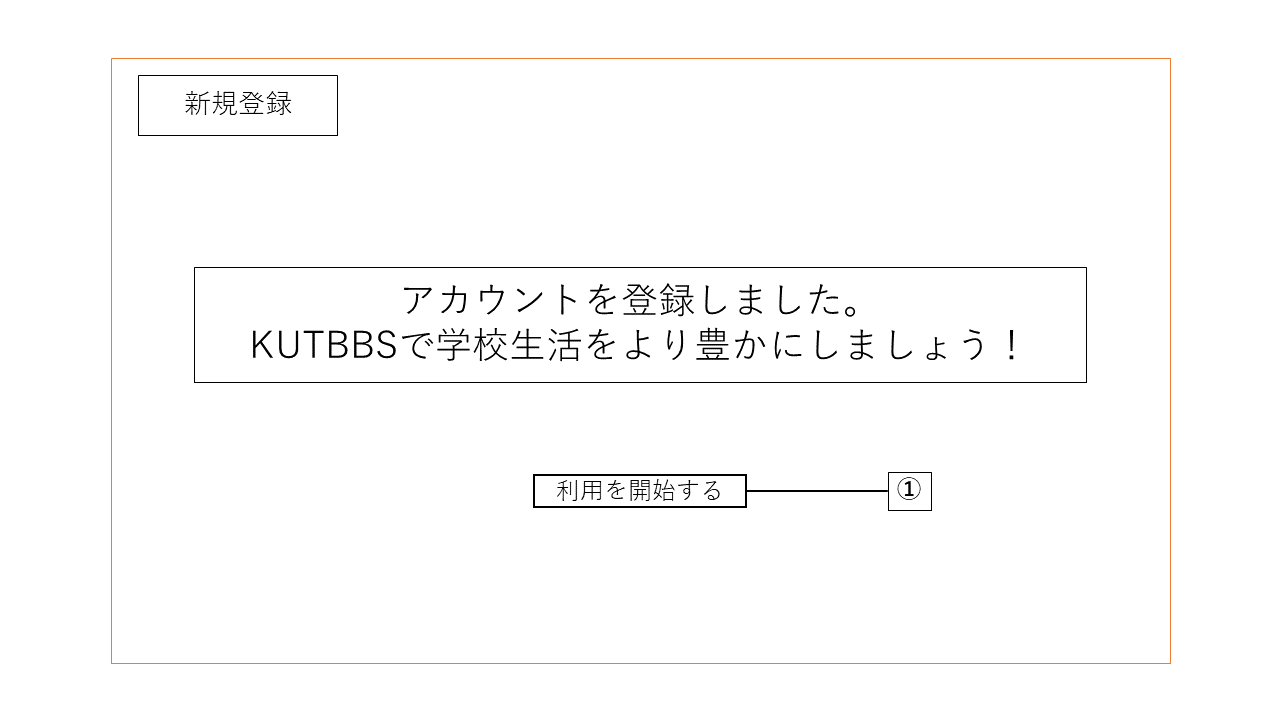
\includegraphics{layout/subscribe_ok.PNG}}
\caption{新規登録確認画面}
\label{fig:subscribe_ok}
\end{figure}

\begin{enumerate}
  \renewcommand{\labelenumi}{\textcircled{\scriptsize \theenumi}}
  \item 利用開始ボタン\\
  利用開始ボタンを押すと、図\ref{fig:BBS_top}に示す掲示板の総合TOP画面に遷移する。
\end{enumerate}

\subsubsection{スティッキーヘッダー}
図\ref{fig:header}に、スティッキーヘッダーの画面を示す。この領域は、ログイン後の他の画面においても常に表示される(送信完了画面と確認画面は除く)、画面をスクロールしても、常に画面上部の表示されている領域である。

\begin{figure}[H]
\centering
\resizebox{14cm}{!}{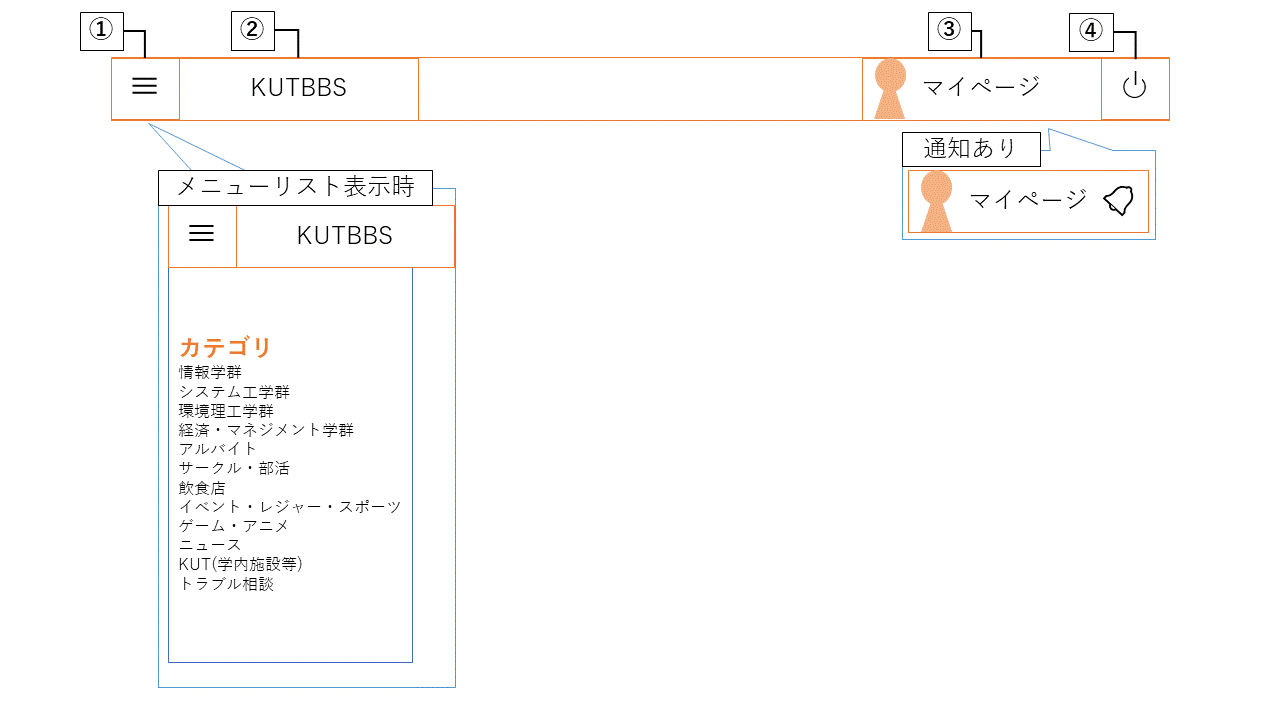
\includegraphics{layout/header.PNG}}
\caption{スティッキーヘッダー}
\label{fig:header}
\end{figure}

\begin{enumerate}
  \renewcommand{\labelenumi}{\textcircled{\scriptsize \theenumi}}

  \item メニューリスト\\
  左端の「≡」マーク(ハンバーガーメニュー)を押すことでカテゴリ一覧を表示する領域である。メニューリストを展開すると、カテゴリ一覧が表示される。任意のカテゴリを押すと、そのカテゴリのTOP画面に遷移する。
  \item ロゴボタン\\
  「KUTBBS」のロゴボタンを押すことで、図\ref{fig:BBS_top}に示す掲示板の総合TOP画面に遷移する。
  \item マイページボタン\\
  マイページサブシステムと通知サブシステムが実装されている領域である。人型アイコン付きのマイページボタンを押すと、図\ref{fig:mypage}に示すマイページに遷移する。また、ユーザに対する通知が合った場合、「マイページ」の文字の隣にベルマークが出現する。
  \item ログアウトボタン\\
  ログインサブシステムが実装されている領域である。電源マークのログアウトボタンを押すことで本システムからログアウトする。
\end{enumerate}


\subsubsection{掲示板の総合TOP画面}
図\ref{fig:BBS_top}に、掲示板の総合TOP画面を示す。この画面は、ユーザが本システムにログインした際に最初に表示される画面である。この画面では、お知らせの閲覧、スレッド検索、カテゴリの選択などを行うことができる。

\begin{figure}[H]
\centering
\resizebox{14cm}{!}{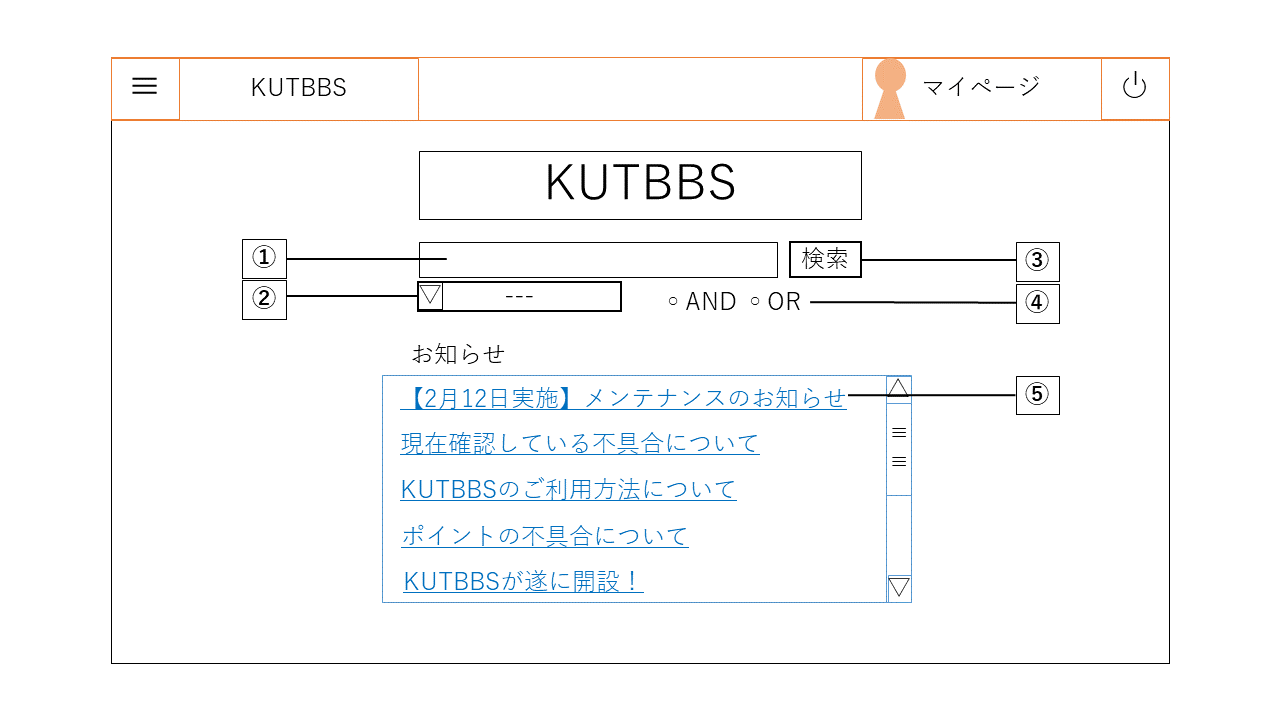
\includegraphics{layout/BBS_top.PNG}}
\caption{掲示板TOP画面}
\label{fig:BBS_top}
\end{figure}

\begin{enumerate}
  \renewcommand{\labelenumi}{\textcircled{\scriptsize \theenumi}}

  \item キーワード入力テキストボックス\\
  検索したいキーワードの入力を行うためのテキストボックスである。
  \item カテゴリ指定ボタン\\
  検索サブシステムが実装されている領域である。検索する際にカテゴリを指定し、そのカテゴリ内のスレッドのみから検索する。
  \item 検索ボタン\\
  検索サブシステムが実装されている領域である。キーワード入力テキストボックスに入力された任意のキーワードに関するスレッドを検索し、図\ref{fig:search_result}に示す検索結果画面に遷移する。
  \item AND/ORボタン\\
  検索サブシステムが実装されている領域である。検索する際にAND検索かOR検索を選択するボタンである。
  \item お知らせ\\
  お知らせ表示サブシステムが実装されている領域である。管理者からのお知らせタイトルを表示する。任意のお知らせタイトルを選択すると、そのお知らせの詳細ページに遷移する。
\end{enumerate}

\subsubsection{カテゴリTOP画面}
図\ref{fig:category_top}にカテゴリTOP画面を示す。この画面は、カテゴリ毎のスレッド一覧を表示するためのもので、任意のカテゴリを選択した際に表示される画面である。
\begin{figure}[H]
\centering
\resizebox{14cm}{!}{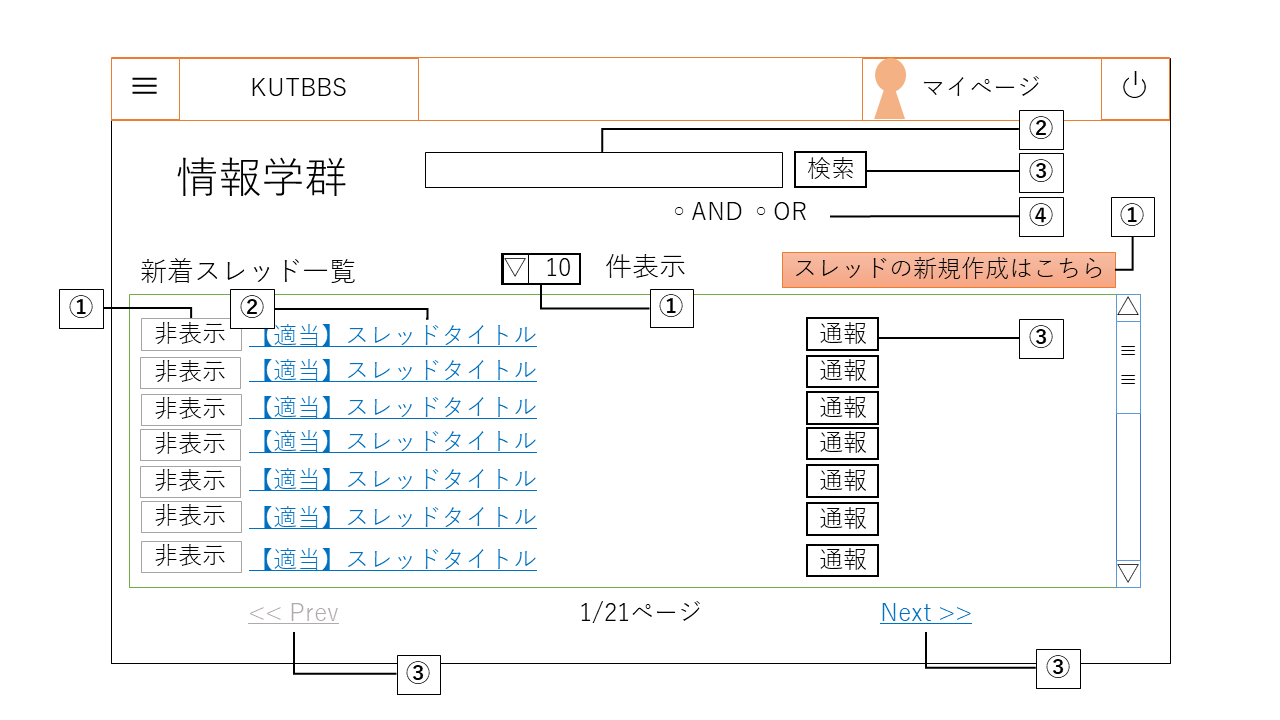
\includegraphics{layout/category_top.PNG}}
\caption{カテゴリTOP画面}
\label{fig:category_top}
\end{figure}
\begin{enumerate}
  \renewcommand{\labelenumi}{\textcircled{\scriptsize \theenumi}}

\item キーワード入力テキストボックス\\
検索したいキーワードの入力を行うためのテキストボックスである。
\item 検索ボタン\\
検索サブシステムが実装されている領域である。キーワードを入力し検索ボタンを押すことで図\ref{fig:search_result}に示す検索結果画面に遷移する。
\item AND/ORボタン\\
検索する際にAND検索かOR検索を選択するボタンである。
\item スレッド新規作成ボタン\\
掲示板サブシステムが実装されている領域である。新規作成ボタンを押すことで図\ref{fig:make_thread}に示すスレッドの新規作成画面へと遷移する。
\item 非表示ボタン(管理者のみ)\\
掲示板編集サブシステムが実装されている領域である。このボタンを押すことで、ユーザが検索した際にそのスレッドタイトルが表示されないようにする。
\item スレッドタイトル\\
掲示板サブシステムが実装されている領域である。スレッドタイトルを選択することでそれに対する図\ref{fig:read_thread}に示すスレッド閲覧画面へと遷移する。
\item 表示件数変換ボタン\\
スレッド一覧の表示件数をユーザが変換できるボタンである。
\item 通報ボタン\\
通報サブシステムが実装されている領域である。通報ボタンを押すことで図\ref{fig:report_reason}通報画面へと遷移する。
\item Prevボタン\\
新着スレッド一覧の前ページを表示する。
\item Nextボタン\\
新着スレッド一覧の次ページを表示する。

\end{enumerate}

\subsubsection{検索結果画面}
図\ref{fig:search_result}に検索結果画面を示す。この画面は、掲示板TOPまたはカテゴリ別TOP画面から検索を行った結果の画面である。
\begin{figure}[H]
\centering
\resizebox{14cm}{!}{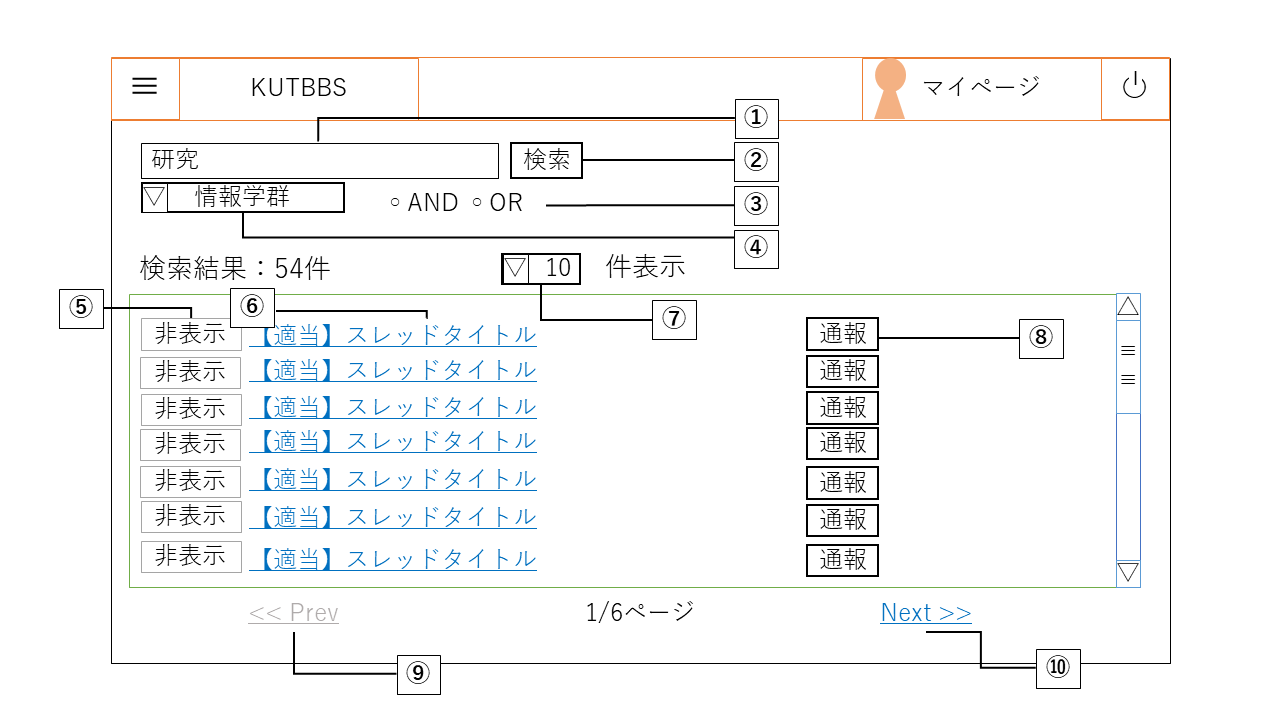
\includegraphics{layout/search_result.PNG}}
\caption{検索結果画面}
\label{fig:search_result}
\end{figure}
\begin{enumerate}
  \renewcommand{\labelenumi}{\textcircled{\scriptsize \theenumi}}

\item キーワード入力テキストボックス\\
検索したいキーワードの入力を行うためのテキストボックスである。
\item 検索ボタン\\
検索サブシステムが実装されている領域である。キーワードを入力し検索ボタンを押すことで再検索を行う。
\item AND/ORボタン\\
検索サブシステムが実装されている領域である。検索する際にAND検索かOR検索を選択するボタンである。
\item カテゴリ指定ボタン\\
検索サブシステムが実装されている領域である。検索する際にカテゴリを指定し、そのカテゴリ内のスレッドのみから検索する。
\item 非表示ボタン(管理者のみ)\\
掲示板編集サブシステムが実装されている領域である。このボタンを押すことで、ユーザが検索した際にそのスレッドタイトルが表示されないようにする。
\item スレッドタイトル\\
掲示板サブシステムが実装されている領域である。スレッドタイトルを選択することでそれに対するスレッド閲覧画面へと遷移する。
\item 表示件数変換ボタン\\
スレッド一覧の表示件数をユーザが変換できるボタンである。
\item 通報ボタン\\
通報サブシステムが実装されている領域である。通報ボタンを押すことで通報画面へと遷移する。
\item Prevボタン\\
検索結果の前ページを表示する。
\item Nextボタン\\
検索結果の次ページを表示する。

\end{enumerate}

\subsubsection{スレッド閲覧画面}
図\ref{fig:read_thread}に、スレッド閲覧画面を示す。この画面は、掲示板システムに属し、掲示板サブシステムを用いてスレッドを閲覧するためのもので、カテゴリTOP画面または検索結果画面からスレッドタイトルを選択することにより表示される画面である。

なお、管理者のみ、掲示板のレスの情報として書き込んだユーザの学籍番号が確認可能である。

\begin{figure}[H]
\centering
\resizebox{14cm}{!}{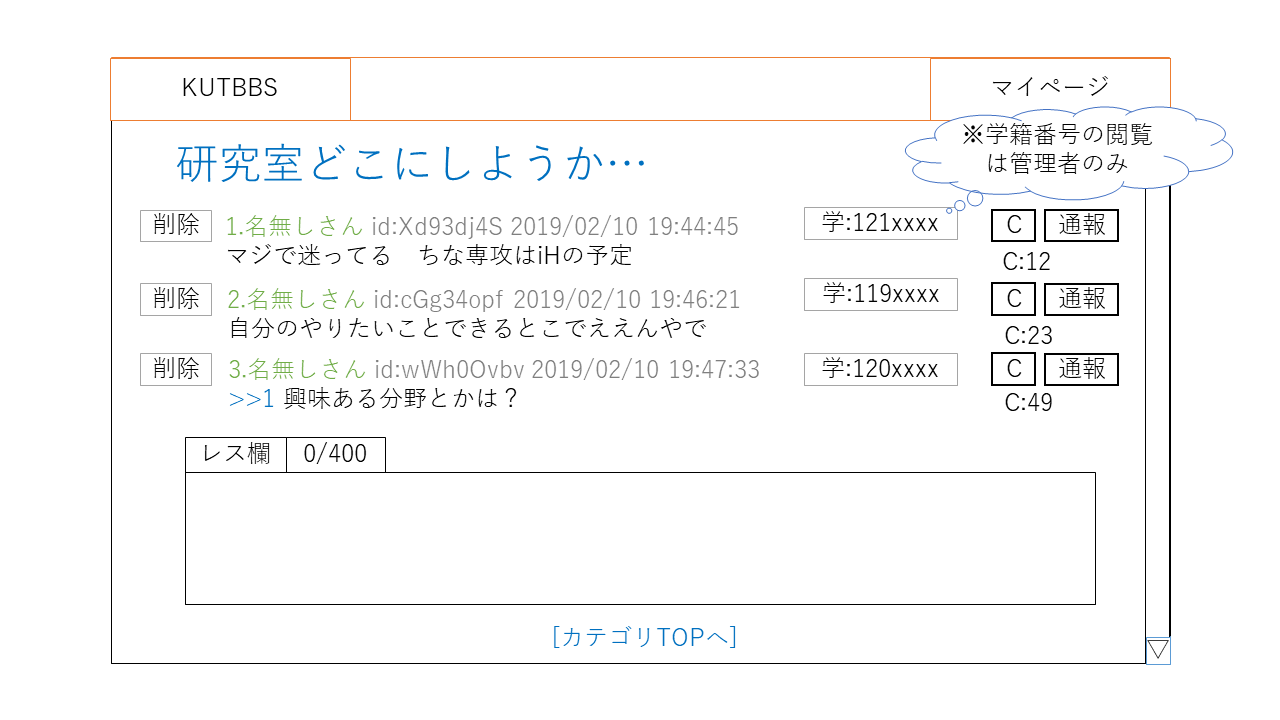
\includegraphics{layout/read_thread.PNG}}
\caption{スレッド閲覧画面}
\label{fig:read_thread}
\end{figure}

\begin{enumerate}
  \renewcommand{\labelenumi}{\textcircled{\scriptsize \theenumi}}
\item 非表示ボタン(管理者のみ)\\
  掲示板編集サブシステムが実装されている領域である。管理者が不適切なレスだと判断したレスを非表示にするためのボタンである。ボタンを押すことでユーザが閲覧する際に、そのレスが表示されないようにする。

\item ブックマークボタン\\
  ブックマークサブシステムが実装されている領域である。このボタンを押すことで、スレッドをブックマークに追加する。

\item 更新ボタン\\
  このボタンを押すことで、スレッドの更新を行う。

\item コレクトボタン\\
  コレクトボタンサブシステムが実装されている領域である。ユーザが特定のレスの情報に信頼性があると感じたときに押すボタンである。

\item 通報ボタン\\
  通報サブシステムが実装されている領域である。ユーザが特定のレスに対して不適切だと感じたときに管理者に報告をするためのボタンである。ボタンを押すと図\ref{fig:report_reason}に示す通報画面へ遷移する。

\item 拡張機能\\
  レスの書き込み時に使用する拡張機能を選択する。

\item レス入力テキストボックス\\
  任意のレスをテキストボックス内に入力する。

\item 送信ボタン\\
  レスを送信するためのボタンである。レス欄が入力された状態で押すことで、図\ref{fig:check_res}に示すレス書き込み確認画面へ遷移する。レス入力テキストボックスに入力されていない場合、エラーメッセージを表示する。

\item カテゴリTOPボタン\\
  このボタンを押すことで、図\ref{fig:category_top}に示すカテゴリTOP画面に遷移する。

\end{enumerate}

\subsubsection{スレッド作成画面}
図\ref{fig:make_thread}に、スレッド作成画面を示す。この画面は、掲示板システムに属し、掲示板サブシステムを用いてスレッドを作成するためのもので、カテゴリTOPからスレッド作成ボタンを押すことにより表示される画面である。\\
\begin{figure}[H]
\centering
\resizebox{14cm}{!}{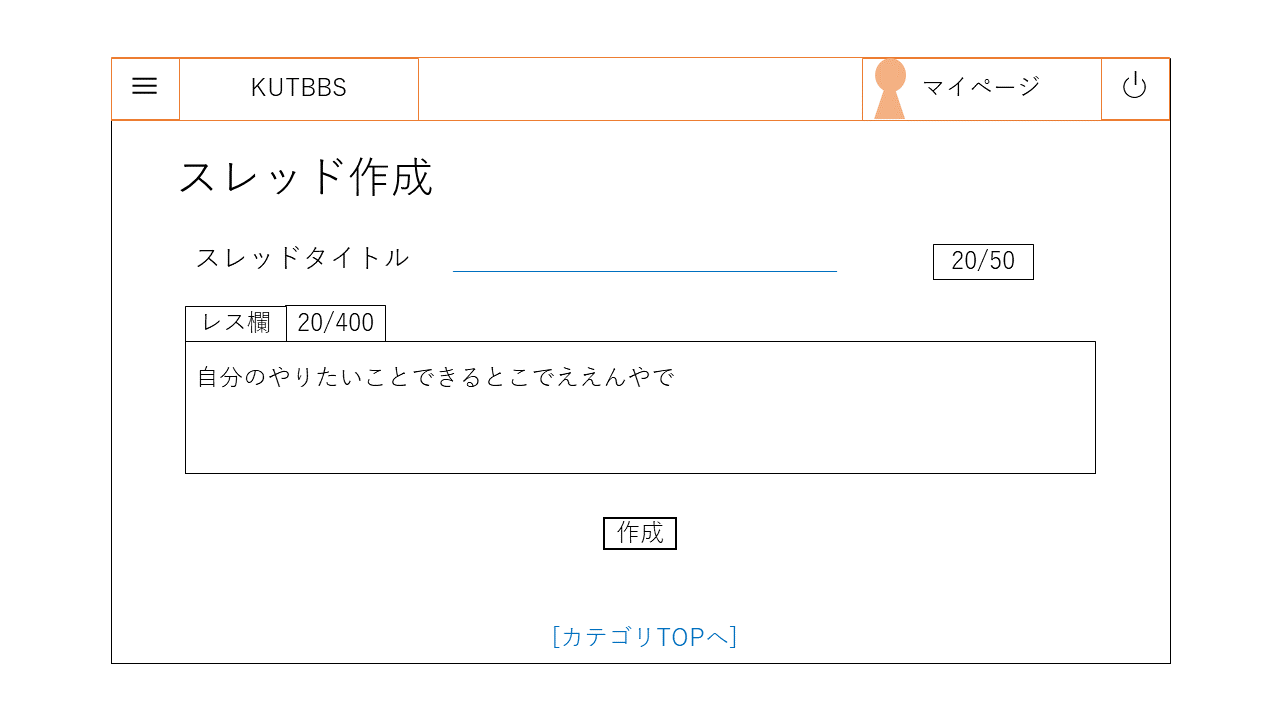
\includegraphics{layout/make_thread.PNG}}
\caption{スレッド作成画面}
\label{fig:make_thread}
\end{figure}

\begin{enumerate}
  \renewcommand{\labelenumi}{\textcircled{\scriptsize \theenumi}}

\item スレッドタイトル入力テキストボックス\\
テキストボックスにスレッドタイトルを入力する。

\item 拡張機能\\
レスの書き込み時に使用する拡張機能を選択する。

\item レス欄(レス入力テキストボックス)\\
任意のレスをテキストボックス内に入力する。

\item 作成ボタン\\
スレッドタイトル・レス欄が入力された状態で押すことで、スレッドを作成し、図\ref{fig:category_top}に示すカテゴリTOP画面に遷移する。入力されていない場合、エラーメッセージを表示する。

\item カテゴリTOPボタン\\
  このボタンを押すことで、図\ref{fig:category_top}に示すカテゴリTOP画面に遷移する。

\end{enumerate}

\subsubsection{レス書き込み確認画面}
図\ref{fig:check_res}に、レス書き込み確認画面を示す。この画面は、掲示板システムに属し、掲示板サブシステムを用いてスレッドに書き込むレスを確認するためのもので、スレッド閲覧画面からレス欄のテキストボックスにレスの書き込みを行い、送信ボタンを押すことにより表示される画面である。

\begin{figure}[H]
\centering
\resizebox{14cm}{!}{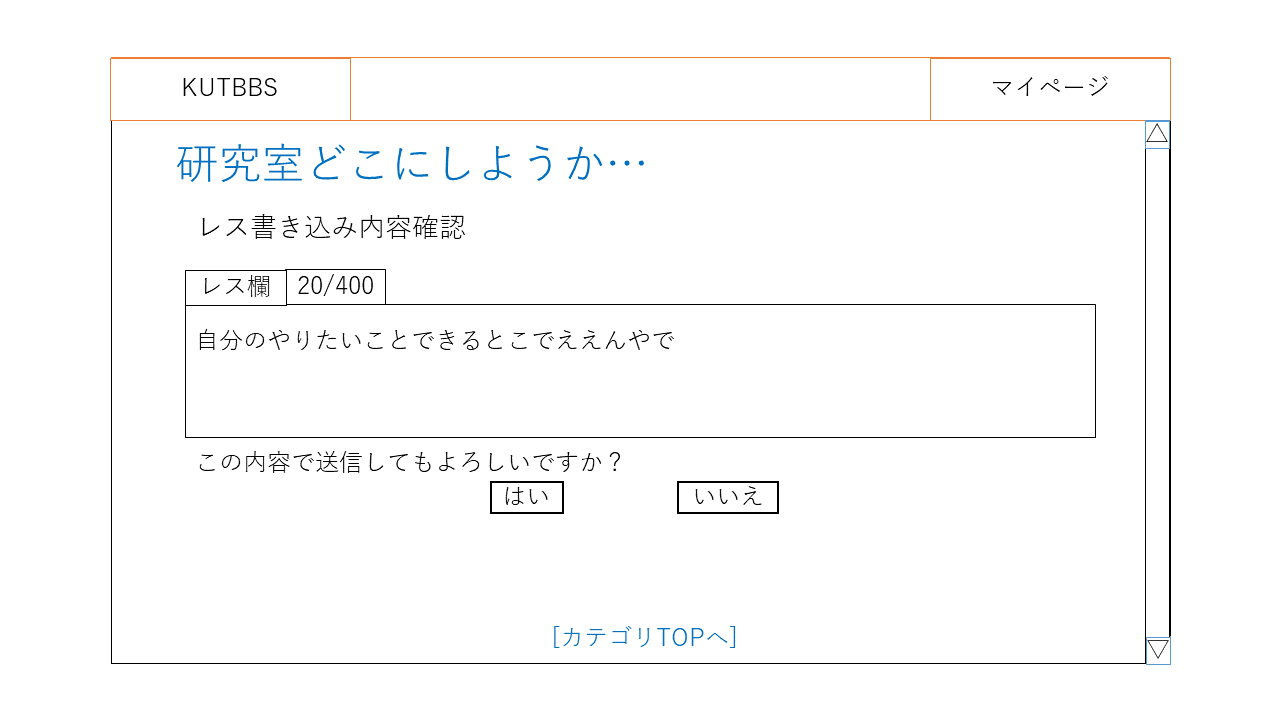
\includegraphics{layout/check_res.PNG}}
\caption{レス書き込み確認画面}
\label{fig:check_res}
\end{figure}

\begin{enumerate}
  \renewcommand{\labelenumi}{\textcircled{\scriptsize \theenumi}}
\item はいボタン\\
  このボタンを押すことで、レスを送信し、レスを書き込んだ後のスレッド閲覧画面に遷移する。
\item いいえボタン\\
  このボタンを押すことで、レスは送信せず、スレッド閲覧画面に遷移する。
\end{enumerate}



\subsubsection{通報画面}
 図\ref{fig:report_reason}はユーザが誹謗中傷や公序良俗に違反するなどの不適切な内容であると判断したスレッドまたはレスを管理者に通報することができる画面である。ユーザは通報理由を文字数400文字以内に記述することができる。「送信」ボタンを押すと通報内容確認画面に遷移する。
\begin{figure}[H]
\begin{center}
\resizebox{14cm}{!}{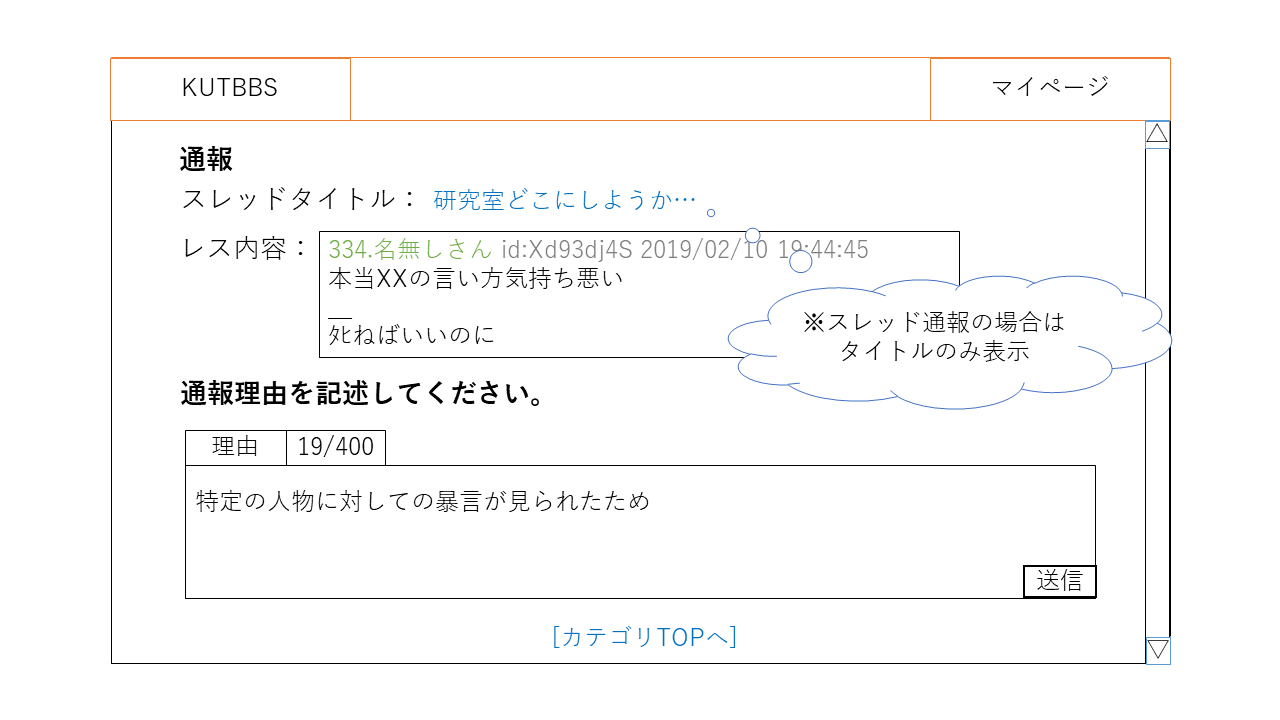
\includegraphics{layout/report_reason.png}}
\caption{通報画面}
\label{fig:report_reason}
\end{center}
\end{figure}

\subsubsection{通報内容確認画面}
図\ref{fig:report_confirm}はユーザが通報画面で記述した内容を確認する画面である。
\begin{figure}[H]
\begin{center}
\resizebox{14cm}{!}{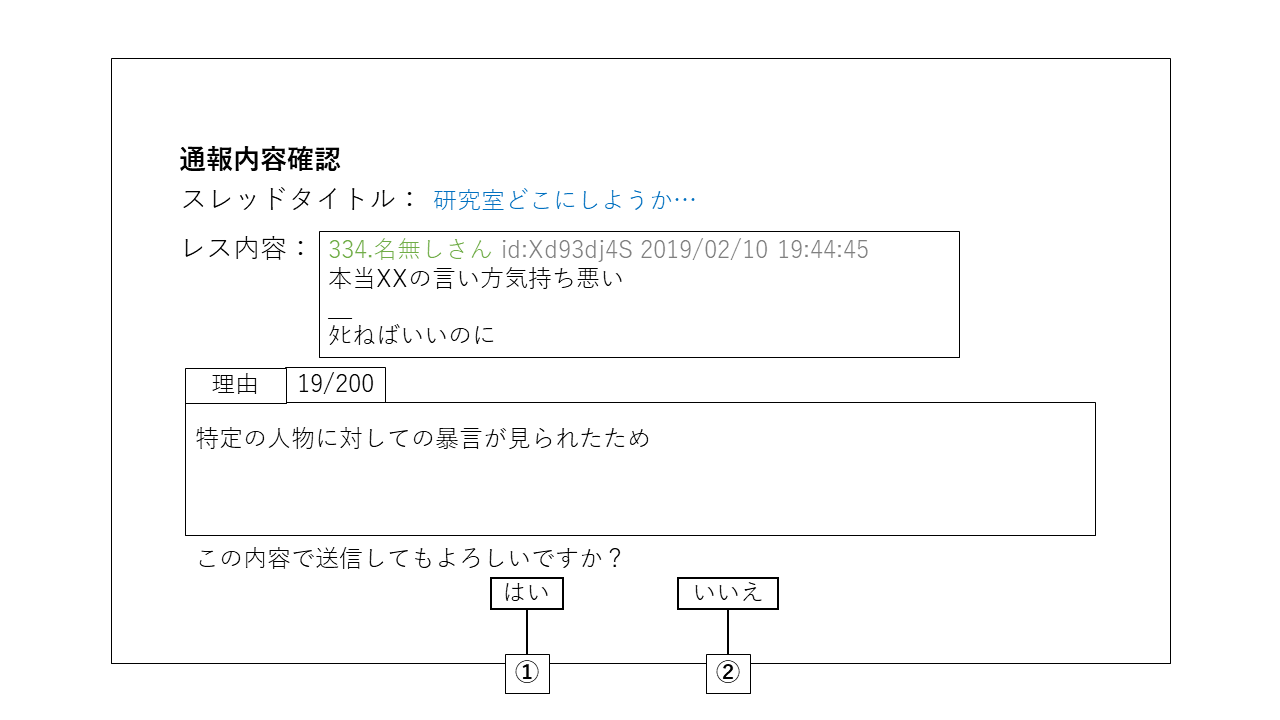
\includegraphics{layout/report_confirm.png}}
\caption{通報内容確認画面}
\label{fig:report_confirm}
\end{center}
\end{figure}

\begin{enumerate}
  \renewcommand{\labelenumi}{\textcircled{\scriptsize \theenumi}}
\item はいボタン\\
  このボタンを押すことで、通報内容を管理者に送信し。図\ref{fig:report_ok}に示す通報内容送信完了画面に遷移する。
\item いいえボタン\\
  このボタンを押すことで、通報画面に戻る。
\end{enumerate}


\subsubsection{通報送信完了画面}
図\ref{fig:report_ok}はユーザが管理者側に通報を送信完了した画面である。
\begin{figure}[H]
\begin{center}
\resizebox{14cm}{!}{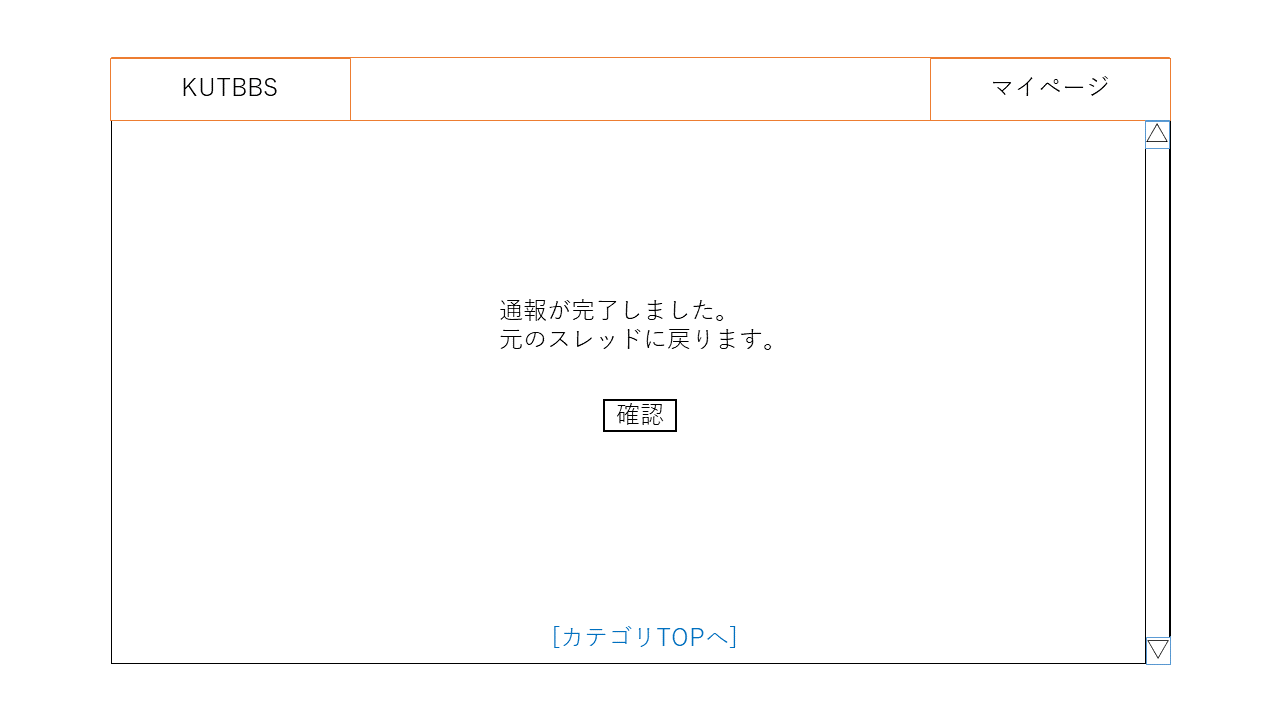
\includegraphics{layout/report_ok.png}}
\caption{通報送信完了画面}
\label{fig:report_ok}
\end{center}
\end{figure}

\begin{enumerate}
  \renewcommand{\labelenumi}{\textcircled{\scriptsize \theenumi}}
\item 戻るボタン\\
このボタンを押すと、カテゴリTOP画面に遷移する。
\end{enumerate}


\subsubsection{マイページ画面}
図\ref{fig:mypage}に、マイページ画面を示す。この画面はユーザ個人のページであり、各種設定を行う。\\

\begin{figure}[H]
\centering
\resizebox{14cm}{!}{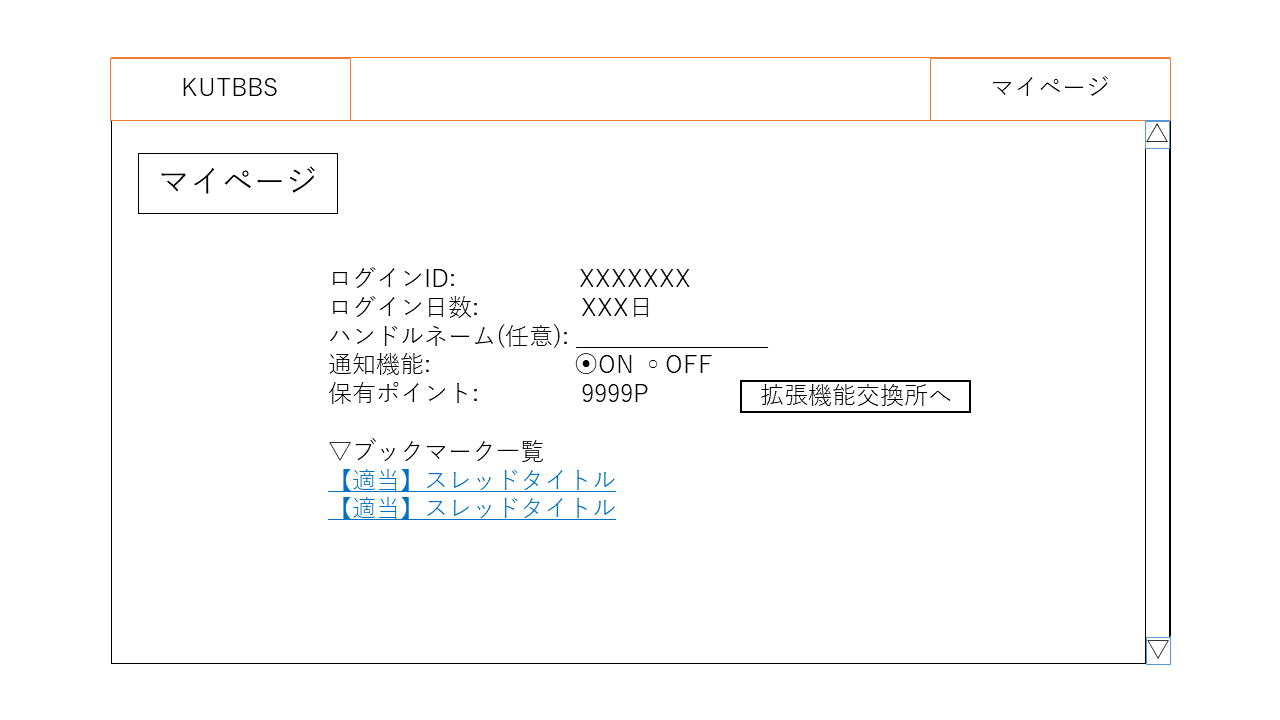
\includegraphics{layout/mypage.PNG}}
\caption{マイページ画面}
\label{fig:mypage}
\end{figure}

\begin{enumerate}
  \renewcommand{\labelenumi}{\textcircled{\scriptsize \theenumi}}

  \item ログインID\\
  各ユーザのログインIDを表示する領域である。
  \item ログイン日数\\
  各ユーザが本システムにログインした累計日数を表示する領域である。
  \item ハンドルネーム\\
  掲示板に表示されるハンドルネームの設定をする領域である。何も設定されていない場合、掲示板には「名無し」と表示される。
  \item 通知設定\\
  通知機能のON/OFFの設定をする領域である。
  \item 保有ポイント\\
  各ユーザが現在所持しているポイントを表示する領域である。
  \item 拡張機能\\
  保有ポイントを消費して掲示板で使用可能な拡張機能を解放することができる領域である。拡張機能の項目は「太字」、「赤字」、「斜体」、「取り消し線」の4つであるが、今後の仕様変更で追加する可能性がある。
  \item ブックマーク一覧\\
  登録したブックマークの一覧を表示する領域である。「ブックマーク一覧」を選択すると展開され、ブックマークの一覧が表示される。
  \item 警告・注意喚起確認ボタン\\
  このボタンを押すと、図\ref{fig:read_warning}に示す警告・注意喚起画面に遷移するボタンである。管理者から警告や注意喚起があった場合、ボタン上に通知を示すベルマークが出現する。
\end{enumerate}

\subsubsection{警告・注意喚起画面}
図\ref{fig:read_warning}に、警告・注意喚起画面を示す。この画面は、管理者からの警告や注意喚起の詳細を確認するためのものである。\\

\begin{figure}[H]
\centering
\resizebox{14cm}{!}{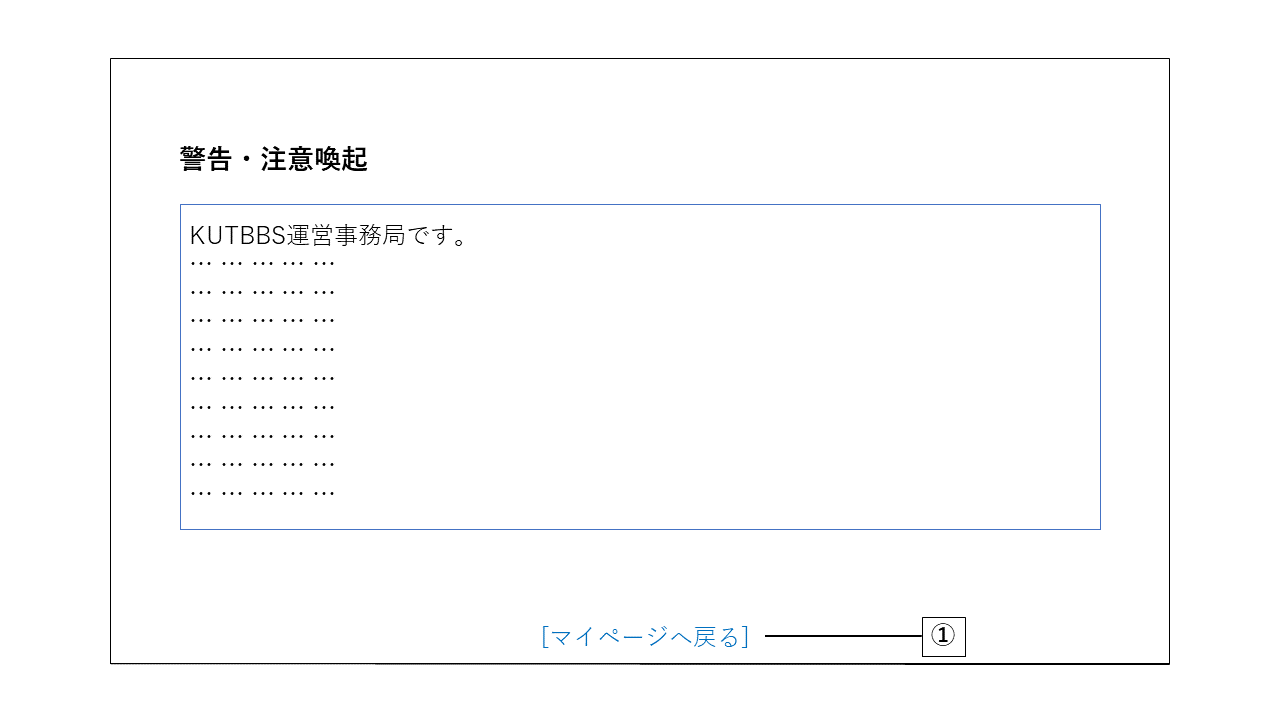
\includegraphics{layout/read_warning.PNG}}
\caption{警告・注意喚起画面}
\label{fig:read_warning}
\end{figure}
\begin{enumerate}
  \renewcommand{\labelenumi}{\textcircled{\scriptsize \theenumi}}

  \item マイページへ戻るボタン\\
  このボタンを押すことで、マイページ画面に遷移する。
\end{enumerate}

\subsection{画面詳細(管理者ページ)}
管理者ページの画面詳細について記す。各図に示す番号と対応させる形式で、画面内のボタン等の持つ詳細な役割を示す。


\subsubsection{管理者ログイン}
図\ref{fig:login_admin}に管理者ログイン画面を示す。この画面は管理者ページの最初に表示される画面であり、本システムの編集を行う管理者であるかの認証を行う。
\begin{figure}[H]
\centering
\resizebox{14cm}{!}{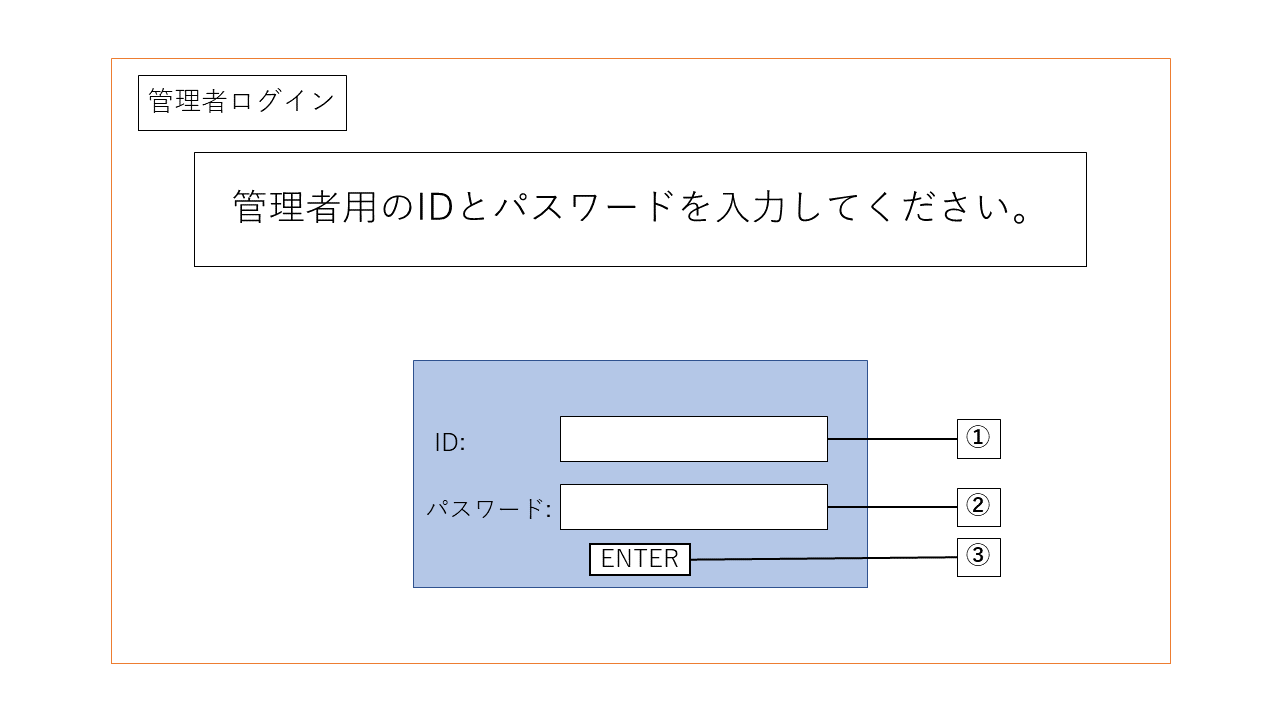
\includegraphics{layout/login_admin.PNG}}
\caption{管理者ログイン}
\label{fig:login_admin}
\end{figure}
\begin{enumerate}
  \renewcommand{\labelenumi}{\textcircled{\scriptsize \theenumi}}

\item ID入力テキストボックス\\
データベースに登録されているIDをテキストボックス内に入力する。
\item パスワード入力テキストボックス\\
データベースに登録されているIDと対応したパスワードをテキストボックス内に入力する。
\item ENTERボタン\\
テキストボックスに入力されたIDとパスワードがデータベースに登録されている場合、ENTERボタンを押すことで管理者トップ画面へと遷移する。入力していない欄がある場合や、入力した内容が一致しなかった場合、エラーメッセージが表示される。

\end{enumerate}


\subsubsection{管理者TOP画面}
図\ref{fig:admin_top}に管理者TOP画面を示す。この画面は、管理者システムに属し、管理者として管理を行うための画面である。\\
管理者は、ユーザ管理・お知らせ編集・通報状況確認・不適切な単語登録を行うことができ、親管理者のみ子管理者管理を行うことができる。

\begin{figure}[H]
\centering
\resizebox{14cm}{!}{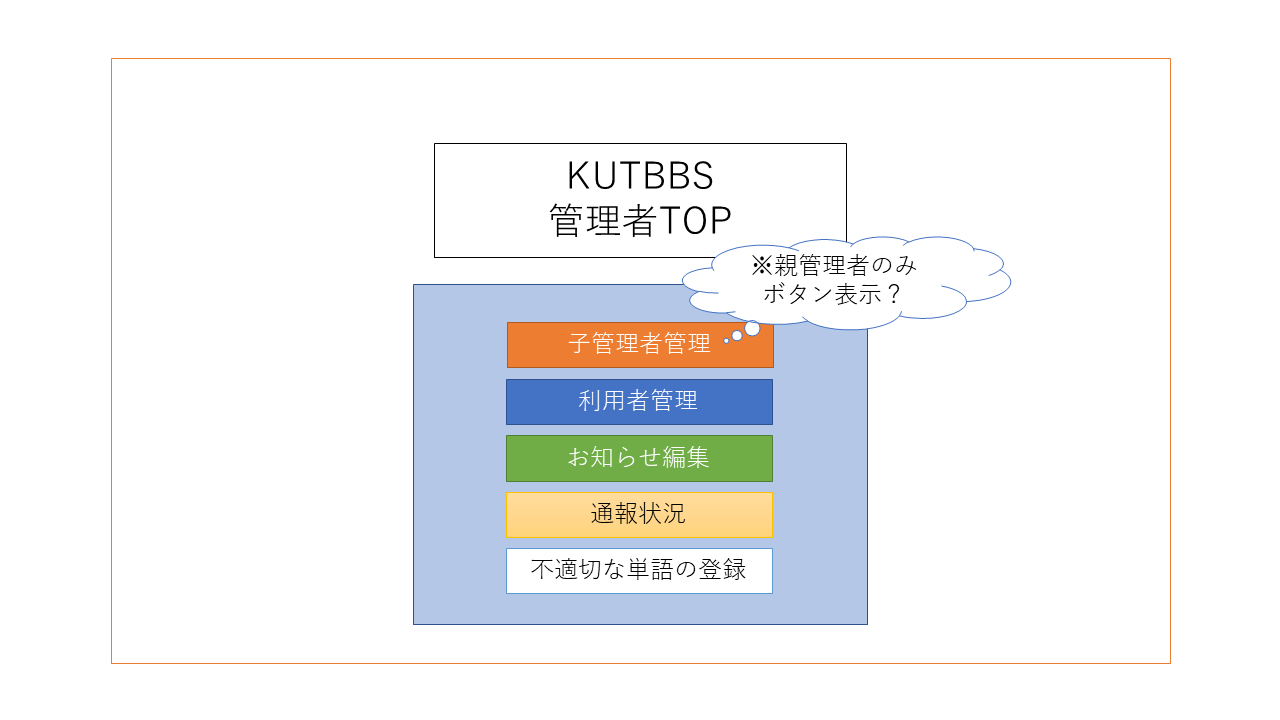
\includegraphics{layout/admin_top.PNG}}
\caption{管理者TOP画面}
\label{fig:admin_top}
\end{figure}
\begin{enumerate}
  \renewcommand{\labelenumi}{\textcircled{\scriptsize \theenumi}}

\item 掲示板TOPはこちらボタン\\
このボタンを押すことで、掲示板の総合TOP画面に遷移する。

\item 子管理者管理ボタン\\
このボタンを押すことで、子管理者管理TOP画面に遷移する。

\item ユーザ管理ボタン\\
このボタンを押すことで、ユーザ管理TOP画面に遷移する。

\item お知らせ編集ボタン\\
このボタンを押すことで、お知らせ編集画面に遷移する。

\item 通報状況確認ボタン\\
このボタンを押すことで、通報状況確認画面に遷移する。

\item 不適切な単語登録ボタン\\
このボタンを押すことで、不適切な単語登録画面に遷移する。
\end{enumerate}

\subsubsection{子管理者管理TOP}
図\ref{fig:admin_child_top}に、子管理者管理TOP画面を示す。この画面は、本システムに登録されている子管理者のIDとパスワードを一覧で表示し、親管理者が子管理者のアカウント管理を行う。

\begin{figure}[H]
\centering
\resizebox{14cm}{!}{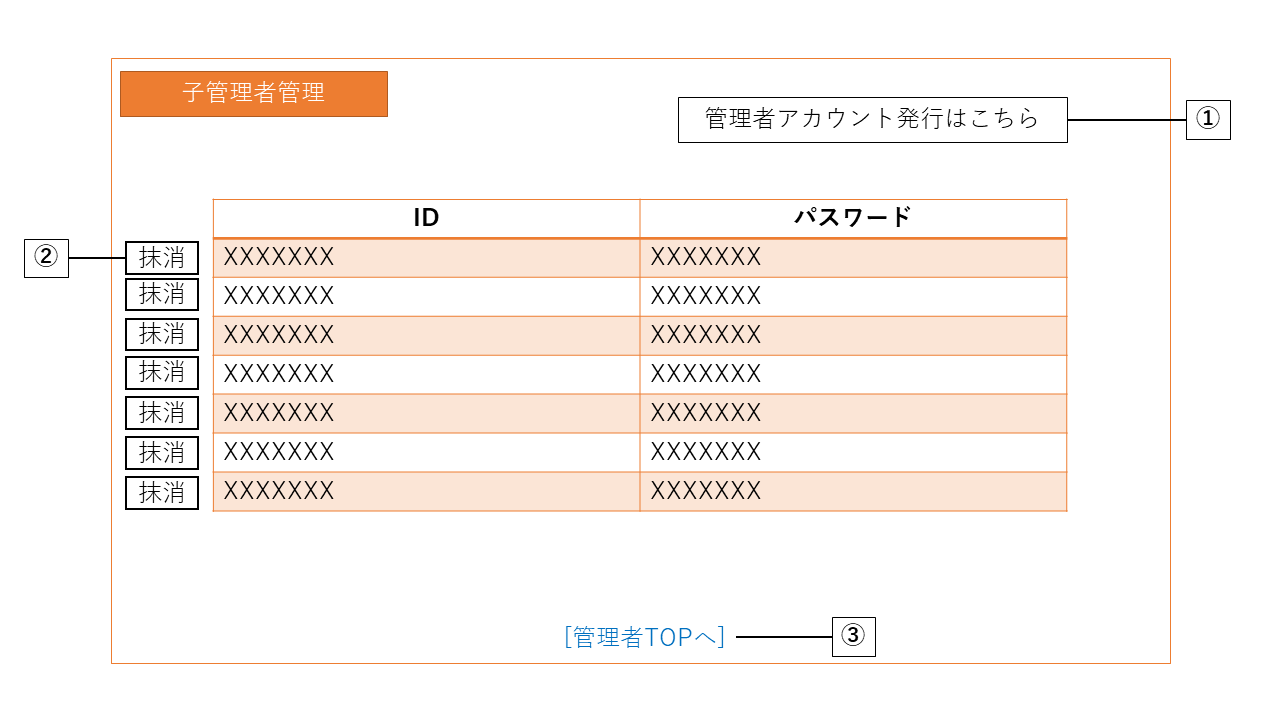
\includegraphics{layout/admin_child_top.PNG}}
\caption{子管理者管理TOP}
\label{fig:admin_child_top}
\end{figure}
\begin{enumerate}
  \renewcommand{\labelenumi}{\textcircled{\scriptsize \theenumi}}

  \item 子管理者アカウント発行ボタン\\
  子管理者を新たに登録する場合、このボタンを押すと、子管理者アカウント発行画面に遷移する。
  \item 子管理者抹消ボタン\\
  現在登録されている任意の子管理者を抹消するボタンである。
  \item 管理者TOPボタン\\
  管理者TOPに遷移するボタンである。

\end{enumerate}

\subsubsection{子管理者アカウント発行画面}
子管理者アカウント発行ボタンを押した場合、図\ref{fig:create_admin}の画面に遷移する。ここで新規で子管理者のアカウントを発行するか否かを選択する。
\begin{figure}[H]
\centering
\resizebox{14cm}{!}{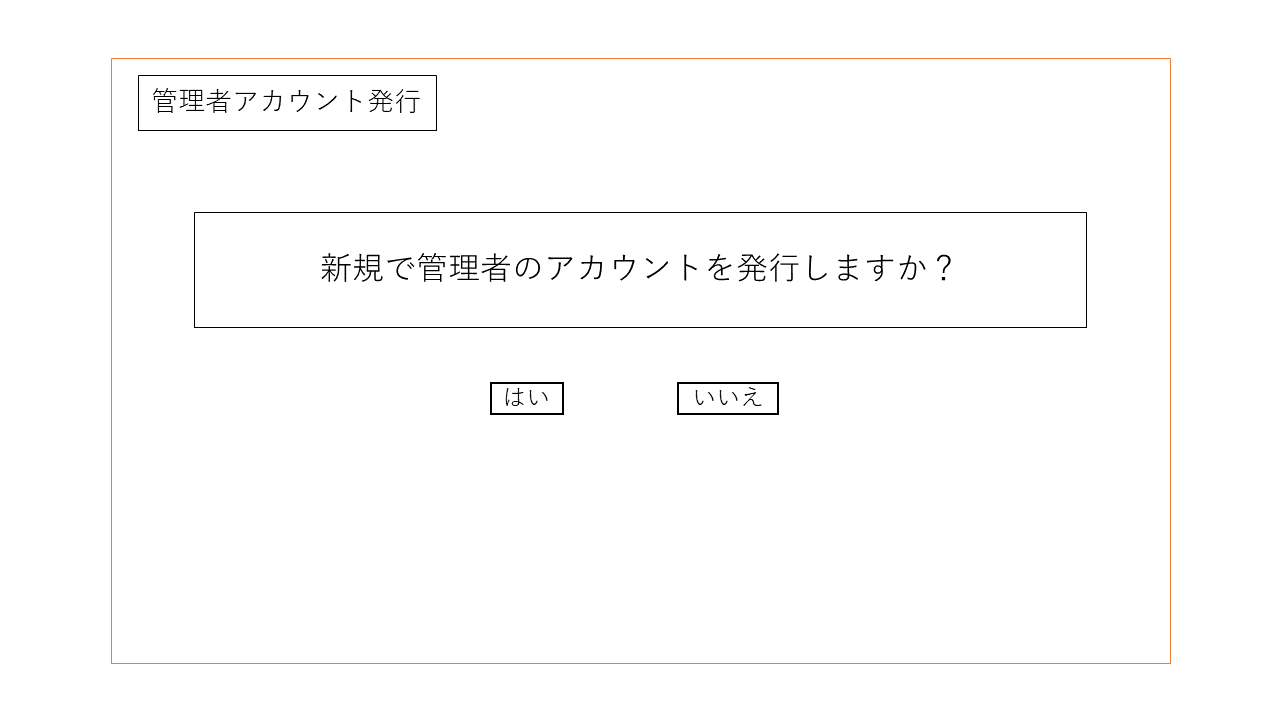
\includegraphics{layout/create_admin.PNG}}
\caption{子管理者アカウント発行画面}
\label{fig:create_admin}
\end{figure}

\begin{enumerate}
  \renewcommand{\labelenumi}{\textcircled{\scriptsize \theenumi}}
\item はいボタン\\
  このボタンを押すことで、子管理者アカウント発行完了画面に遷移する。
\item いいえボタン\\
  このボタンを押すことで、子管理者管理TOP画面に遷移する。
\end{enumerate}

\subsubsection{子管理者アカウント発行画面}
図\ref{fig:create_admin}で「はい」を選択すると、図\ref{fig:new_admin}の画面に遷移する。子管理者アカウントの発行が完了したことを表示し、発行したアカウントのIDとパスワードが表示される。

\begin{figure}[H]
\centering
\resizebox{14cm}{!}{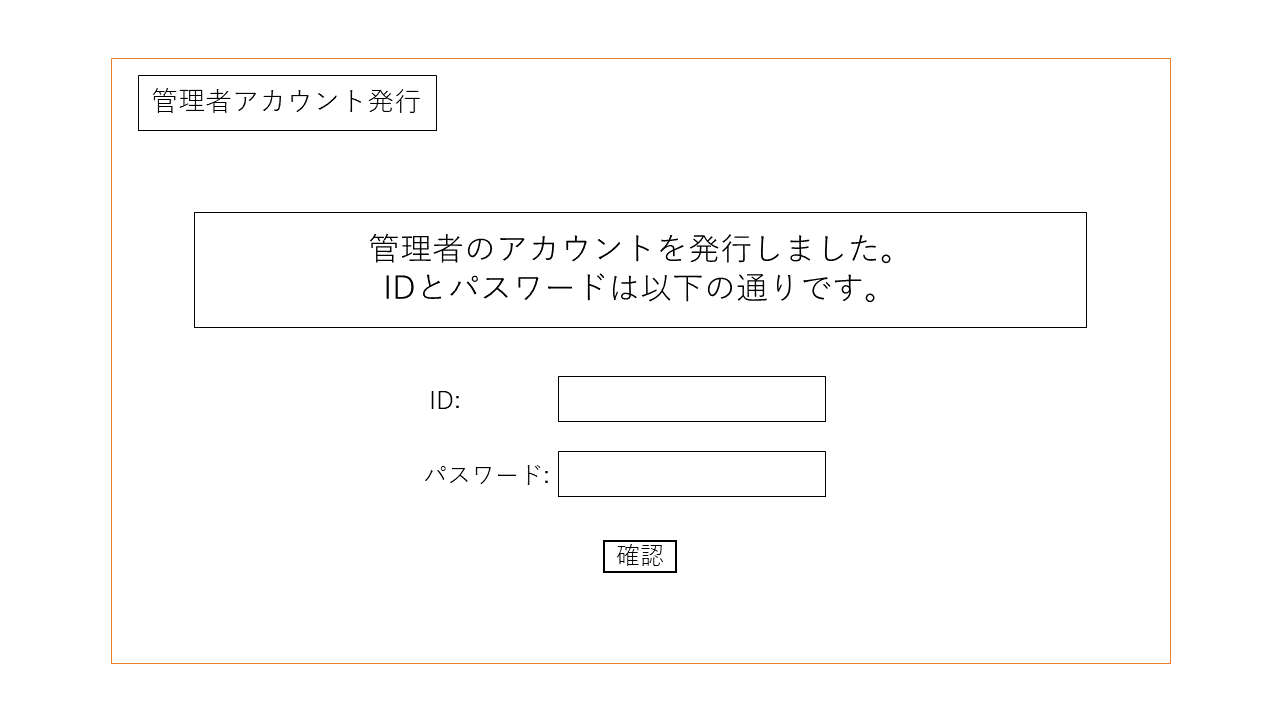
\includegraphics{layout/new_admin.PNG}}
\caption{子管理者アカウント発行完了画面}
\label{fig:new_admin}
\end{figure}

\begin{enumerate}
  \renewcommand{\labelenumi}{\textcircled{\scriptsize \theenumi}}
\item 確認ボタン\\
  このボタンを押すことで、子管理者管理TOP画面に遷移する。
\item 管理者TOPボタン\\
  このボタンを押すことで、管理者TOP画面に遷移する。
\end{enumerate}



\subsubsection{子管理者アカウント抹消画面}
また、図\ref{fig:admin_child_top}で子管理者抹消ボタンを押すと、図\ref{fig:delete_admin}の画面に遷移する。ここで特定の子管理者のアカウントを抹消するか否かを選択する。

\begin{figure}[H]
\centering
\resizebox{14cm}{!}{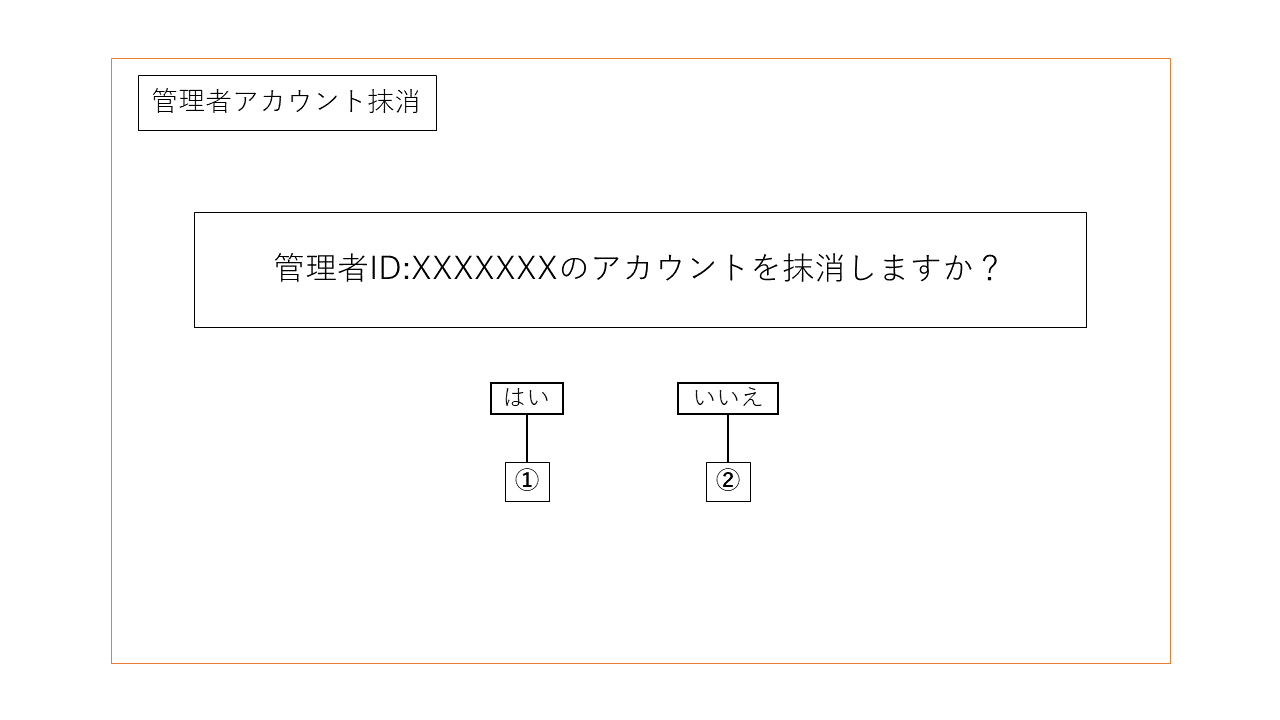
\includegraphics{layout/delete_admin.PNG}}
\caption{子管理者アカウント抹消画面}
\label{fig:delete_admin}
\end{figure}

\begin{enumerate}
  \renewcommand{\labelenumi}{\textcircled{\scriptsize \theenumi}}
\item はいボタン\\
  このボタンを押すことで、子管理者アカウント抹消画面に遷移する。
\item いいえボタン\\
  このボタンを押すことで、子管理者管理TOP画面に遷移する。
\end{enumerate}

\subsubsection{子管理者アカウント抹消完了画面}

図\ref{fig:delete_admin}で「はい」を押すと、図\ref{fig:delete_admin_ok}の画面に遷移する。特定の子管理者アカウントの抹消が完了したことを表示し、「戻る」を選択して子管理者管理TOP画面に遷移する。
\begin{figure}[H]
\centering
\resizebox{14cm}{!}{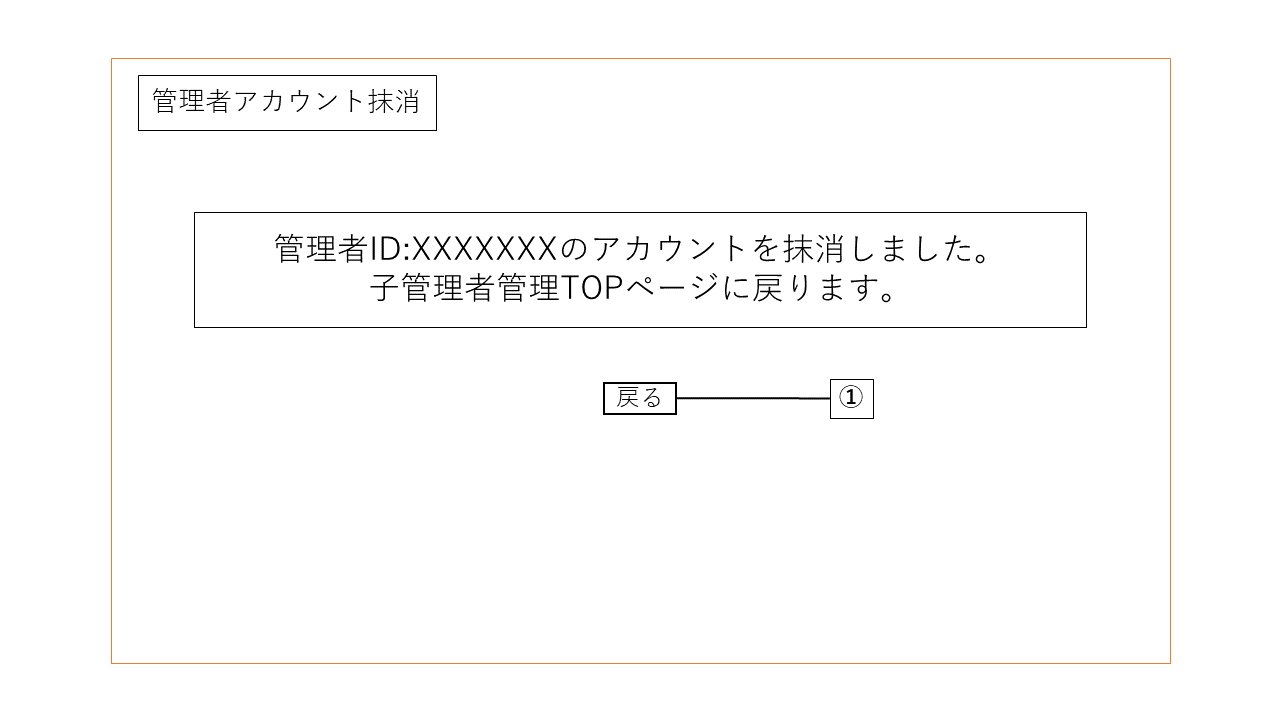
\includegraphics{layout/delete_admin_ok.PNG}}
\caption{子管理者アカウント抹消完了画面}
\label{fig:delete_admin_ok}
\end{figure}

\begin{enumerate}
  \renewcommand{\labelenumi}{\textcircled{\scriptsize \theenumi}}
\item 戻るボタン\\
  このボタンを押すことで、子管理者管理TOP画面に遷移する。
\end{enumerate}



\subsubsection{ユーザ管理画面}
図\ref{fig:user_admin_top}にユーザ管理画面を示す。この画面は、ユーザ管理サブシステムを用いてユーザのアカウント発行とユーザ情報検索を行うことができる。
\begin{figure}[H]
\centering
\resizebox{14cm}{!}{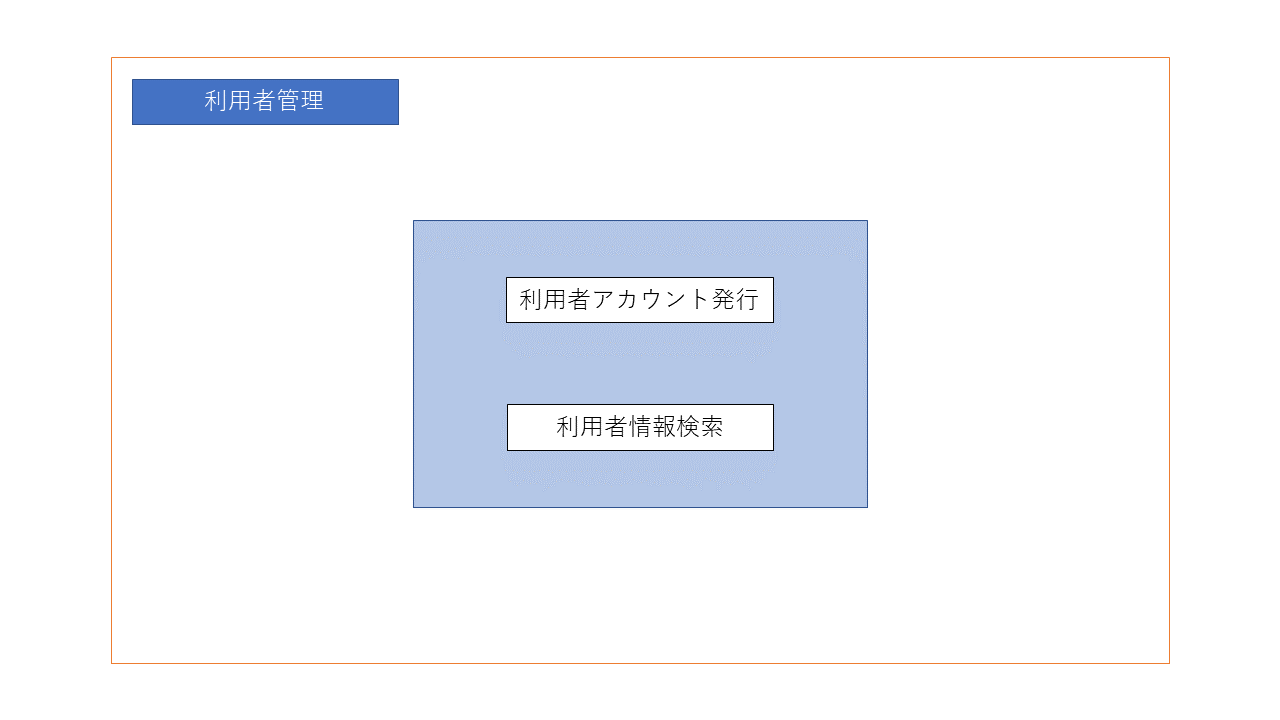
\includegraphics{layout/user_admin_top.PNG}}
\caption{ユーザ管理画面}
\label{fig:user_admin_top}
\end{figure}

\begin{enumerate}
  \renewcommand{\labelenumi}{\textcircled{\scriptsize \theenumi}}

\item ユーザアカウント発行ボタン\\
ユーザ登録サブシステムが実装されている領域である。ユーザアカウント発行ボタンを押すことで、ユーザアカウント発行画面へと遷移する。

\item ユーザ情報検索ボタン\\
ユーザ管理サブシステムが実装されている領域である。ユーザ情報検索ボタンを押すことで、ユーザ情報検索画面に遷移する。

\end{enumerate}

\subsubsection{ユーザアカウント発行画面}
図\ref{fig:create_user}にユーザアカウント発行画面を示す。この画面は、ユーザ登録サブシステムを用いてユーザアカウントの発行を行うことができる。新しく発行するユーザの学籍番号の範囲を入力して、ユーザアカウントの発行を行う。
\begin{figure}[H]
\centering
\resizebox{14cm}{!}{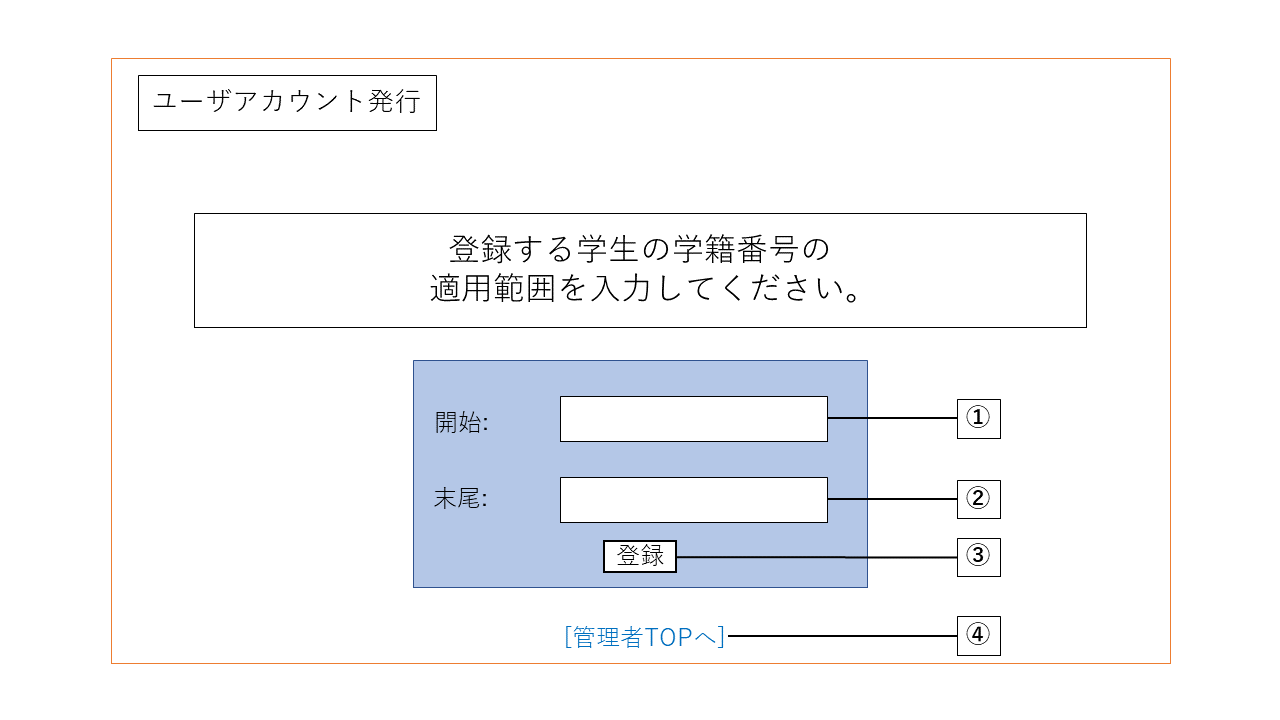
\includegraphics{layout/create_user.PNG}}
\caption{ユーザアカウント発行画面}
\label{fig:create_user}
\end{figure}

\begin{enumerate}
  \renewcommand{\labelenumi}{\textcircled{\scriptsize \theenumi}}

\item 開始番号テキストボックス\\
  新しく発行するユーザの開始番号を入力するテキストボックスである。
\item 末尾番号テキストボックス\\
  新しく発行するユーザの末尾番号を入力するテキストボックスである。
\item 登録ボタン\\
  開始番号テキストボックスに入力された学籍番号と末尾番号テキストボックスに入力された学籍番号の範囲のユーザのアカウントを登録するためのボタンである。
  \item 管理者TOPボタン\\
  このボタンを押すことで、管理者TOP画面に遷移する。
\end{enumerate}

\subsubsection{ユーザアカウント発行確認画面}
図\ref{fig:new_user}にユーザアカウント発行確認画面を示す。この画面は、ユーザアカウントを発行する際の学籍番号の確認を行うことができる。
\begin{figure}[H]
\centering
\resizebox{14cm}{!}{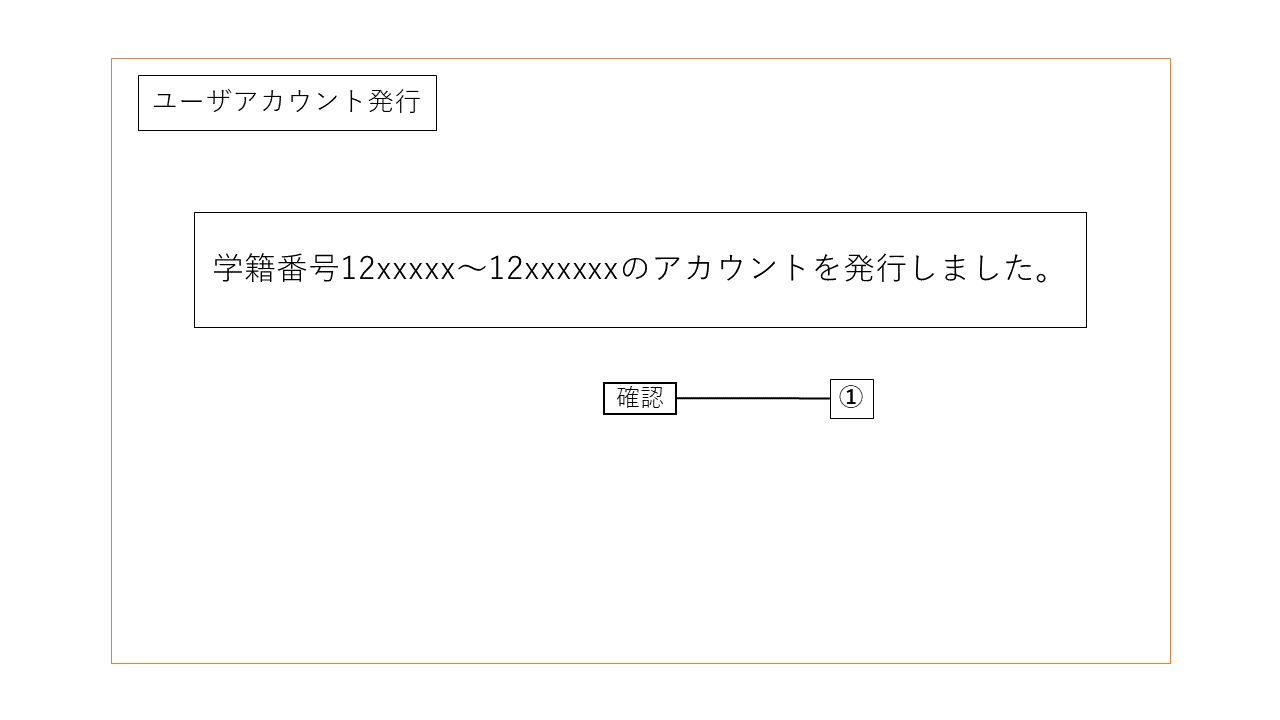
\includegraphics{layout/new_user.PNG}}
\caption{ユーザアカウント発行確認画面}
\label{fig:new_user}
\end{figure}

\begin{enumerate}
  \renewcommand{\labelenumi}{\textcircled{\scriptsize \theenumi}}

\item 確認ボタン\\
確認ボタンを押すとユーザ管理画面に遷移する。

\end{enumerate}

\subsubsection{ユーザ情報検索画面}
図\ref{fig:search_user}にユーザ情報検索画面を示す。この画面は、ユーザ管理サブシステムを用いて管理者がユーザ情報を検索する際に表示する。

\begin{figure}[H]
\centering
\resizebox{14cm}{!}{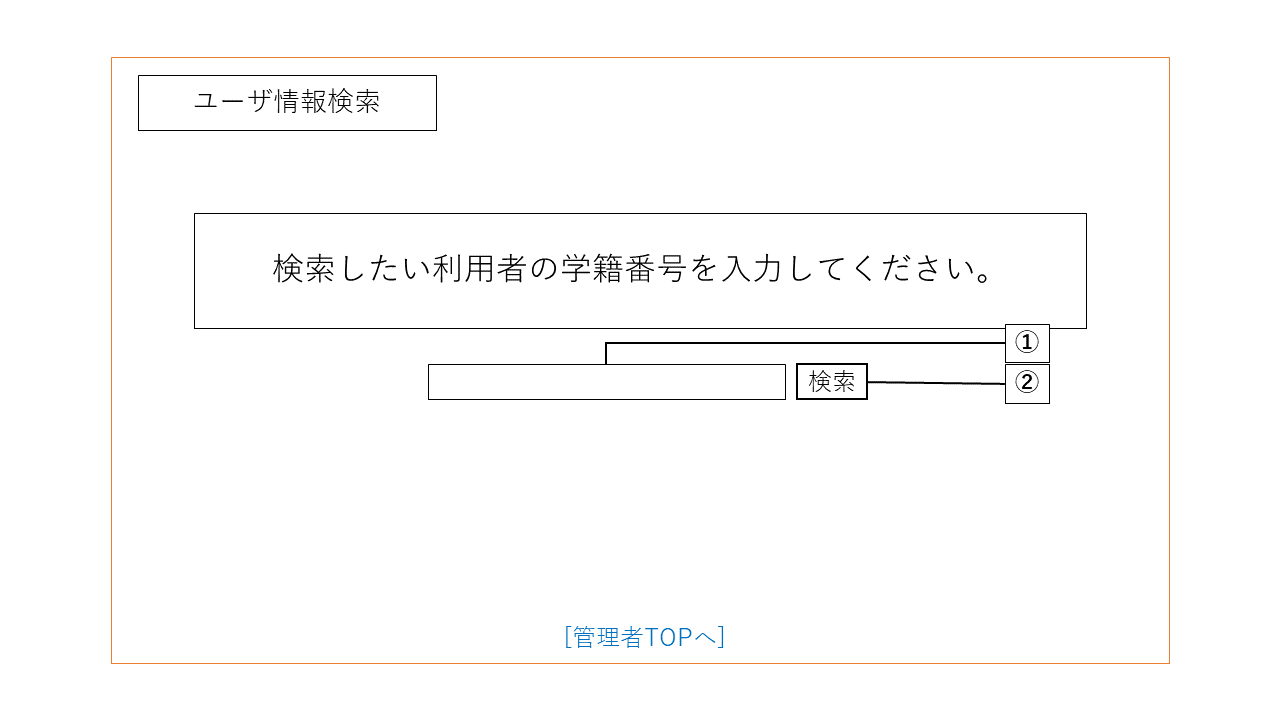
\includegraphics{layout/search_user.PNG}}
\caption{ユーザ情報検索画面}
\label{fig:search_user}
\end{figure}

\begin{enumerate}
  \renewcommand{\labelenumi}{\textcircled{\scriptsize \theenumi}}

\item 学籍番号検索テキストボックス\\
ユーザ管理サブシステムが実装されている領域である。管理者がユーザの情報を入手する際に学籍番号を入力するテキストボックスである。

\item 検索ボタン\\
検索ボタンを押すことで学籍番号検索テキストボックスに入力されている学籍番号に合わせてユーザの検索を行う。その後、検索したユーザ情報画面に遷移する。学籍番号検索テキストボックスに入力していない場合や、入力した内容が一致しなかった場合、エラーメッセージが表示される。


\end{enumerate}


\subsubsection{ユーザ情報画面}
図\ref{fig:user_info}にユーザ情報画面を示す。この画面ではユーザ情報を検索した際に表示され確認を行うことができる。
\begin{figure}[H]
\centering
\resizebox{14cm}{!}{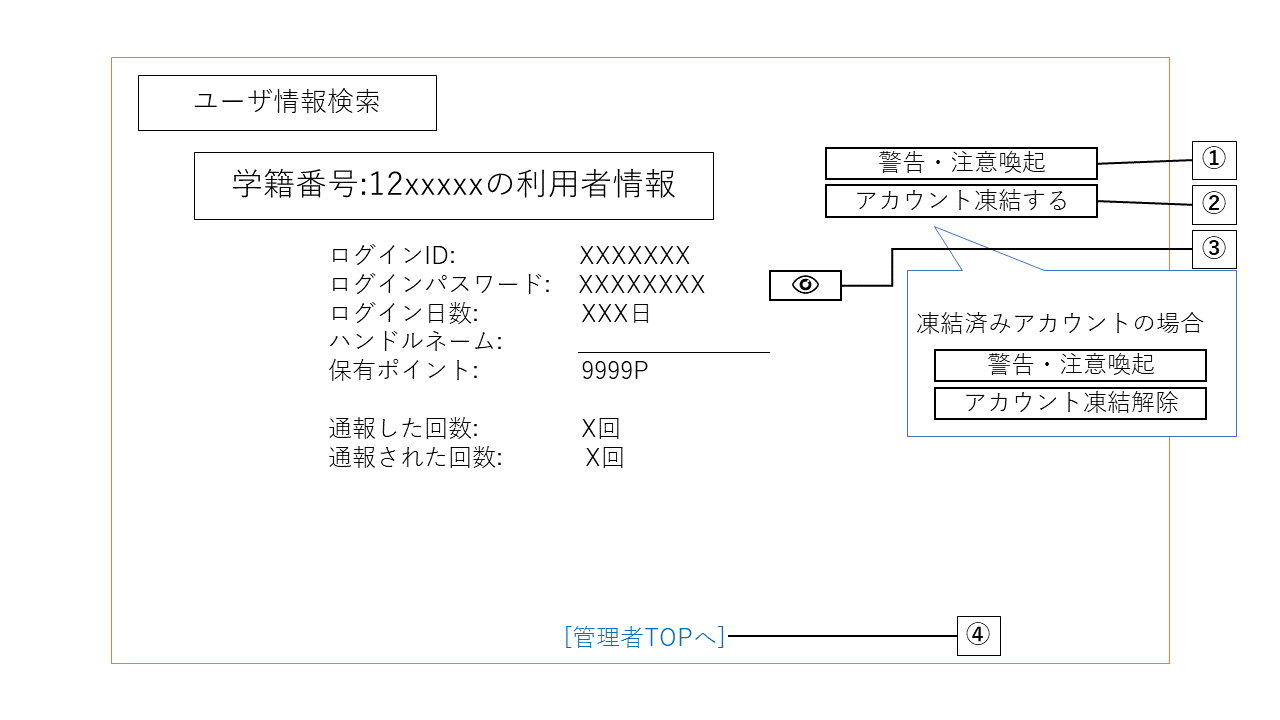
\includegraphics{layout/user_info.PNG}}
\caption{ユーザ管理}
\label{fig:user_info}
\end{figure}

\begin{enumerate}
  \renewcommand{\labelenumi}{\textcircled{\scriptsize \theenumi}}

\item 警告・注意喚起ボタン\\
表示されているユーザに対して、警告・注意喚起を行う際に警告・注意喚起ボタンを押すことで、警告・注意喚起画面に遷移する。
\item アカウント凍結ボタン(アカウント凍結解除ボタン)\\
  ユーザのアカウントを凍結する際にアカウント凍結ボタンを押すことで、アカウントを凍結する。

  ユーザのアカウントが既に凍結されている場合、アカウント凍結解除ボタンとして表示する。アカウント凍結解除ボタンを押すことで、アカウント凍結を解除する。
  \item パスワード表示ボタン\\
  このボタンを押すことで、伏せ字になっているログインパスワードを表示する。再度ボタンを押すことで、パスワードを伏せ字にできる。
  \item 管理者TOPボタン\\
  このボタンを押すことで、管理者TOP画面に遷移する。

\end{enumerate}

\subsubsection{警告・注意喚起画面}
図\ref{fig:warning}に警告・注意喚起画面を示す。この画面ではユーザに対して警告・注意喚起を行う際にメッセージ内容の記述を行うことができる。

\begin{figure}[H]
\centering
\resizebox{14cm}{!}{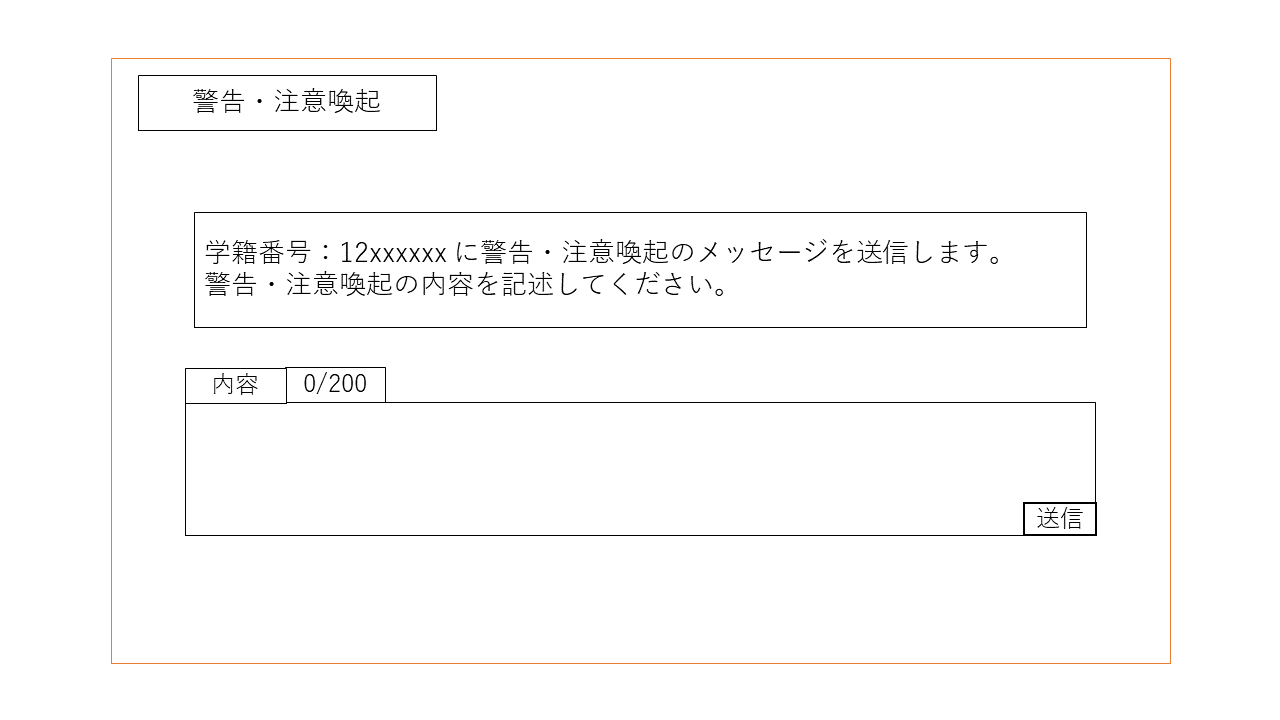
\includegraphics{layout/warning.PNG}}
\caption{警告・注意喚起画面}
\label{fig:warning}
\end{figure}

\begin{enumerate}
  \renewcommand{\labelenumi}{\textcircled{\scriptsize \theenumi}}

\item メッセージ内容テキストボックス\\
ユーザに警告・注意喚起を行うためにメッセージ内容を記述できるテキストボックスである。
\item 送信ボタン\\
  このボタンを押すことで、警告・注意喚起の確認画面へと遷移する。メッセージ内容テキストボックスに入力していない場合、エラーメッセージが表示される。
\item ユーザ情報ページに戻るボタン\\
  このボタンを押すことで、ユーザ情報画面に遷移する。
\end{enumerate}

\subsubsection{警告・注意喚起確認画面}
図\ref{fig:warning_confirm}に警告・注意喚起確認画面を示す。この画面では警告・注意喚起を行う際に記述したメッセージ内容の確認を行うことができる。
\begin{figure}[H]
\centering
\resizebox{14cm}{!}{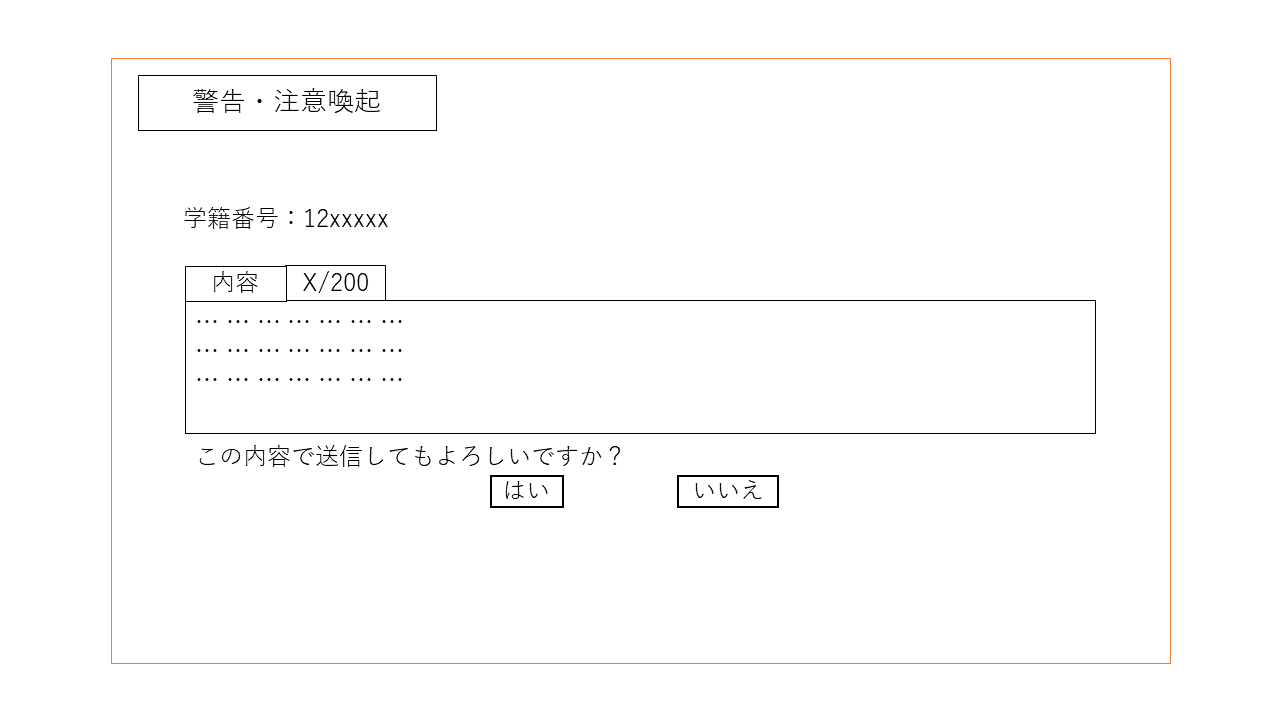
\includegraphics{layout/warning_confirm.PNG}}
\caption{警告・注意喚起画面}
\label{fig:warning_confirm}
\end{figure}

\begin{enumerate}
  \renewcommand{\labelenumi}{\textcircled{\scriptsize \theenumi}}

\item はいボタン\\
メッセージ内容に誤りがない場合に押すことで、警告・注意喚起完了画面へと遷移する。
\item いいえボタン\\
このボタンを押すことで、ユーザ情報ページへと遷移する。
\end{enumerate}

\subsubsection{警告・注意喚起完了画面}
図\ref{fig:warning_ok}に警告・注意喚起完了画面を示す。この画面では警告・注意喚起を行う際のメッセージが送信されたことを確認することができる。
\begin{figure}[H]
\centering
\resizebox{14cm}{!}{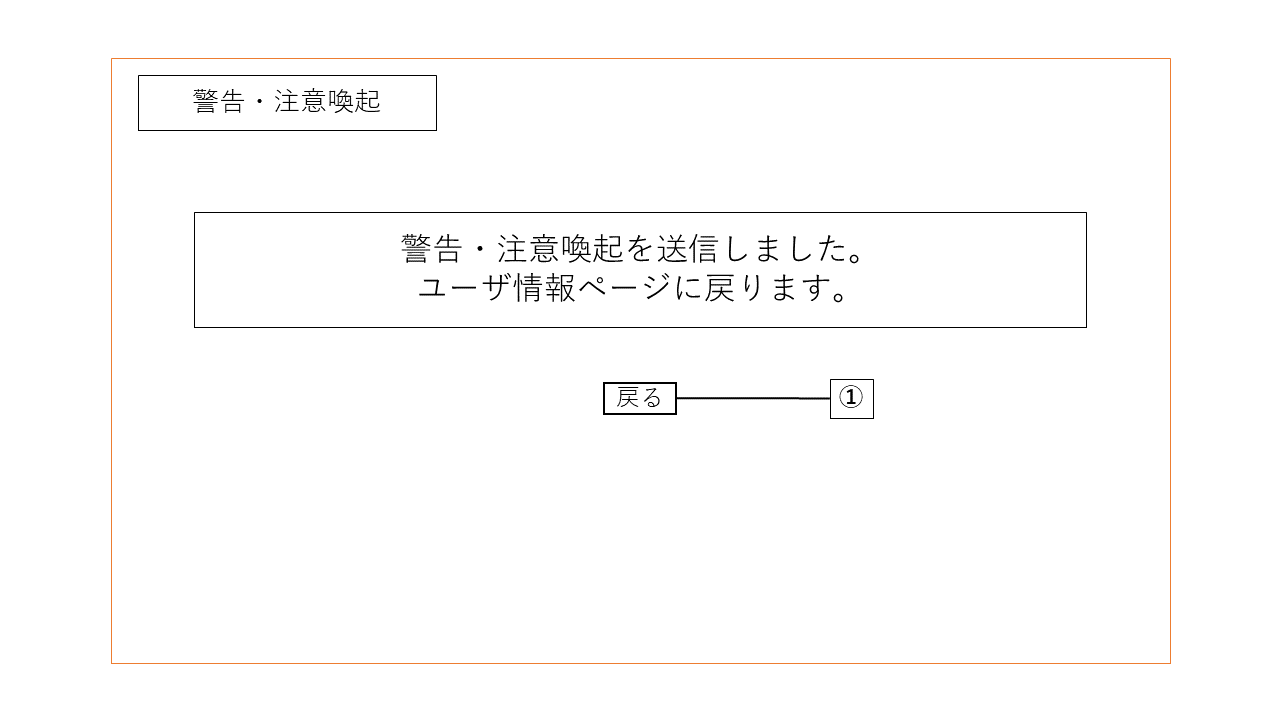
\includegraphics{layout/warning_ok.PNG}}
\caption{警告・注意喚起完了画面}
\label{fig:warning_ok}
\end{figure}

\begin{enumerate}
  \renewcommand{\labelenumi}{\textcircled{\scriptsize \theenumi}}

\item 戻るボタン\\
戻るボタンを押すことでユーザ情報画面へと遷移する。

\end{enumerate}


\subsubsection{通報状況画面}
図\ref{fig:report_admin}はユーザが通報した内容を管理者が閲覧できる画面である。管理者は、ユーザから送られた通報内容を確認を行い、通報状況を見て適切な処置を行うことができる。また、「ユーザ情報検索へ」ボタンを押すことでユーザ情報検索画面へ遷移することができる。
\begin{figure}[H]
\begin{center}
\resizebox{14cm}{!}{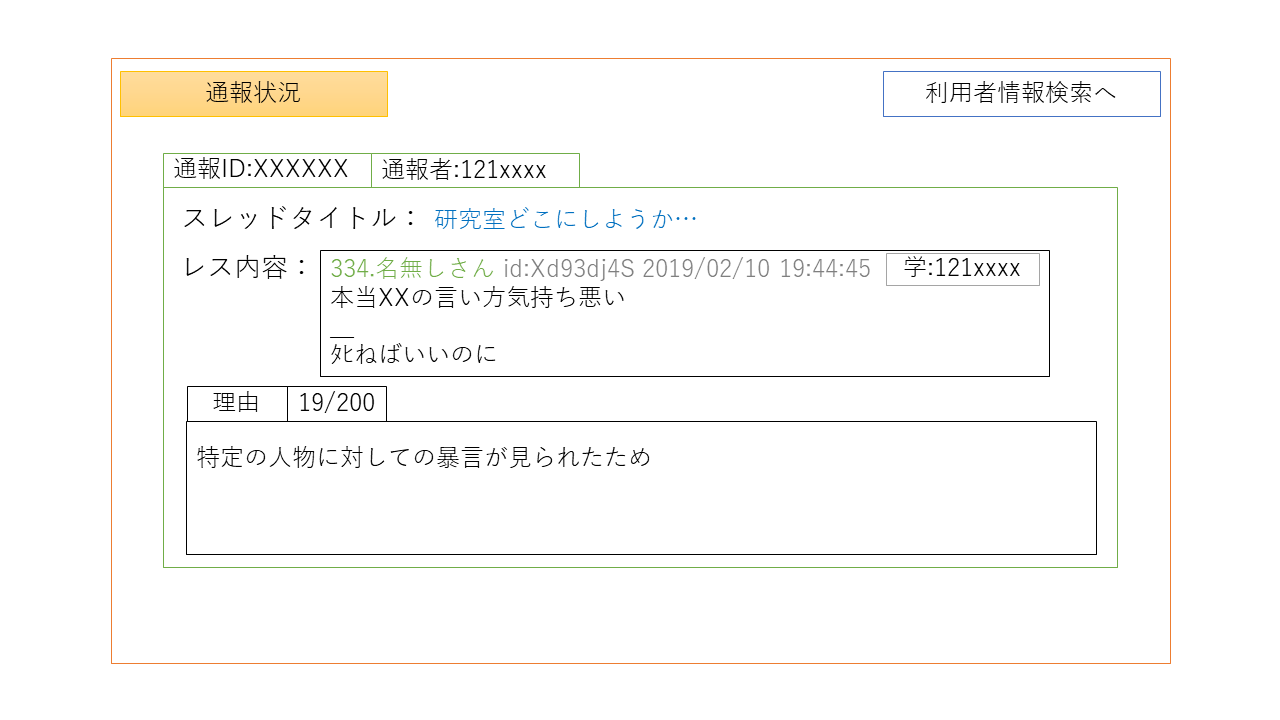
\includegraphics{layout/report_admin.png}}
\caption{通報状況画面}
\label{fig:report_admin}
\end{center}
\end{figure}

\begin{enumerate}
  \renewcommand{\labelenumi}{\textcircled{\scriptsize \theenumi}}

\item ユーザ情報検索ボタン\\
このボタンを押すことで、ユーザ情報検索画面へと遷移する。
\item 非表示ボタン\\
このボタンを押すことで、通報されたレスを掲示板上で非表示する。
\item 通報理由\\
ユーザから通報されたスレッドまたはレスに対する通報理由を表示する領域である。
\item 管理者TOPボタン\\
このボタンを押すことで、管理者TOP画面に遷移する。

\end{enumerate}

\subsubsection{不適切な単語登録画面}
図\ref{fig:NGword}に、不適切な単語の登録画面を示す。この画面では、既に登録されている不適切な単語の閲覧し、新たに不適切な単語を登録する。

図\ref{fig:NGword}に示す番号と対応させる形式で、以下にその役割を示す。
\begin{figure}[H]
\centering
\resizebox{14cm}{!}{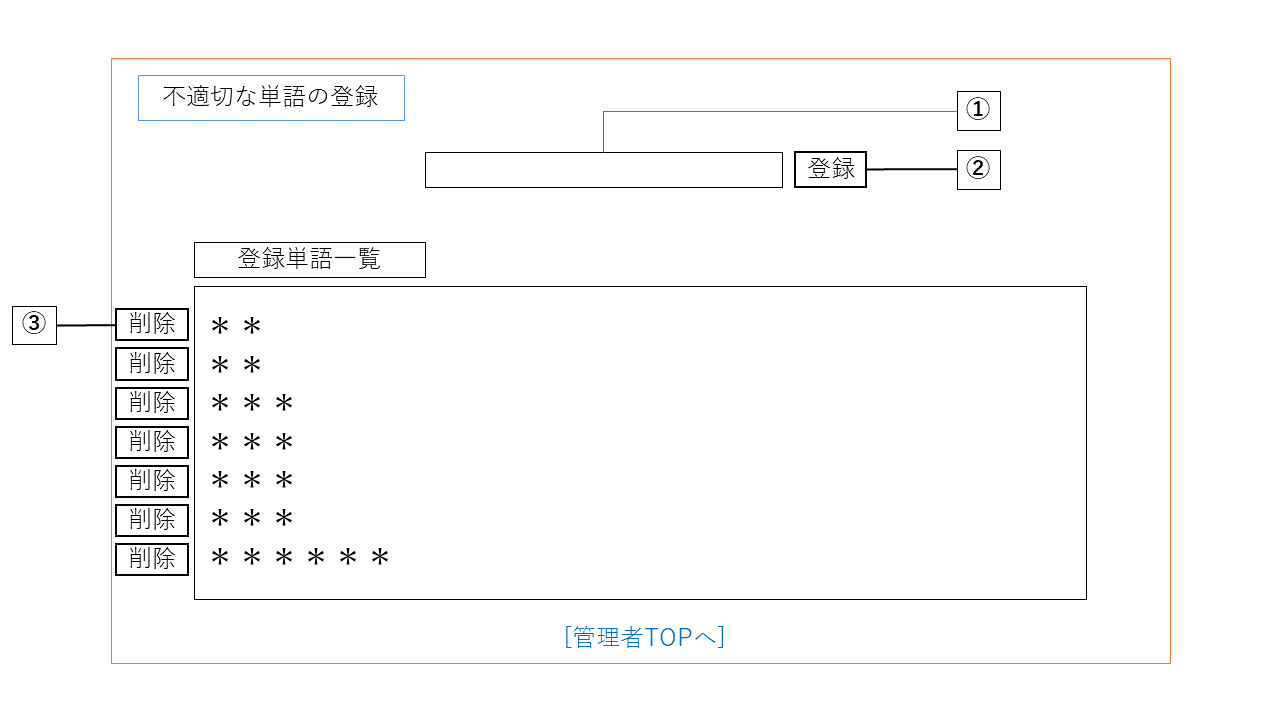
\includegraphics{layout/NGword.PNG}}
\caption{不適切な単語登録画面}
\label{fig:NGword}
\end{figure}
\begin{enumerate}
  \renewcommand{\labelenumi}{\textcircled{\scriptsize \theenumi}}
  \item 不適切な単語入力テキストボックス\\
  新たに登録する不適切な単語を入力する領域である。
  \item 不適切な単語登録ボタン\\
  入力の登録ボタンを押すと、不適切な単語の登録をする。入力テキストボックスに何も入力せずに登録ボタンを押すと、エラーメッセージが表示される。
  \item 削除ボタン\\
  既に登録されている不適切な単語を削除するボタンである。ボタンを押すと、該当単語が削除された状態の不適切な単語登録画面を表示する。
\end{enumerate}

% 不適切な単語入力テキストボックスに、新たに登録する単語を入力した上で登録ボタンを押すと、図\ref{fig:NGword_confirm}の画面に遷移する。入力した単語を確認し、不適切な単語として登録するか否かを選択する。はいボタンを押すと不適切な単語登録完了画面に遷移し、いいえボタンを押すと不適切な単語登録画面に戻る。
% \begin{figure}[H]
% \centering
% \resizebox{14cm}{!}{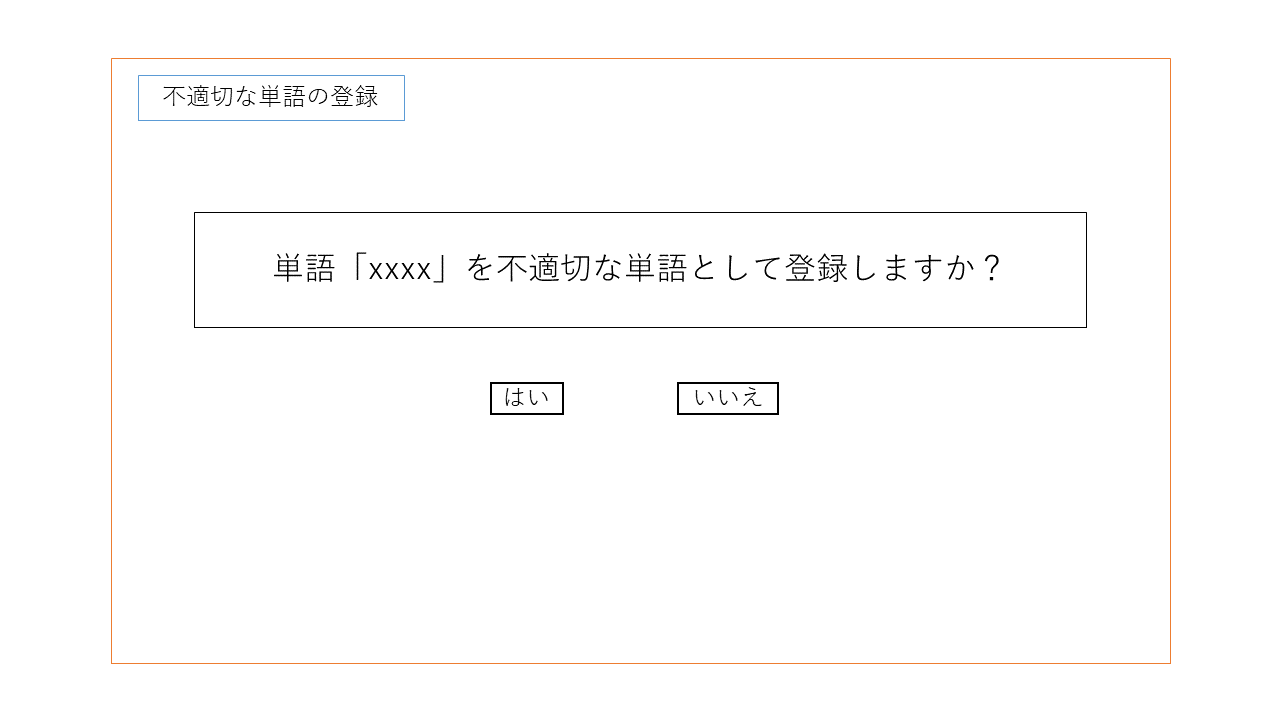
\includegraphics{layout/NGword_confirm.PNG}}
% \caption{不適切な単語登録確認画面}
% \label{fig:NGword_confirm}
% \end{figure}
% 不適切な単語登録確認画面ではいボタンを押すと、図\ref{fig:NGword_ok}の画面に遷移する。単語の登録が完了したことを表示し、「戻る」ボタンを選択して不適切な単語の登録ページに遷移する。
% \begin{figure}[H]
% \centering
% \resizebox{14cm}{!}{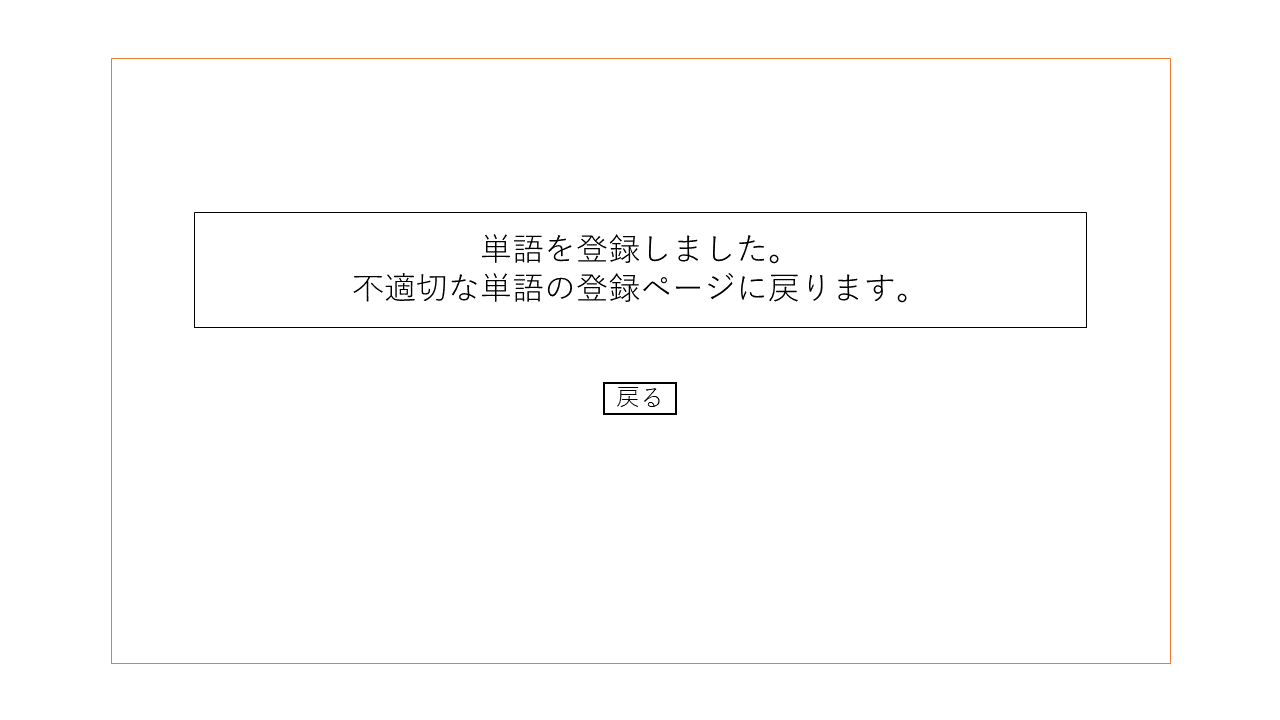
\includegraphics{layout/NGword_ok.PNG}}
% \caption{不適切な単語登録完了画面}
% \label{fig:NGword_ok}
% \end{figure}

\section{データベース設計}
本システムに用いるデータベースはMySQLを用いて、データベースの仕様、データベースの構造を示す。
\subsection{データテーブル仕様}
本システムのデータベースには、9個のデータテーブルが存在する。各データテーブルの仕様をデータモデルを用いて以下に示す。
\begin{itemize}
\item ユーザテーブル\\
  ユーザテーブルでは本システムを利用するユーザに関する情報を管理する。またフラグを用いることでユーザと管理者(親管理者と子管理者)を区別、拡張機能の付与、初回ログインの判別を行っている。表1にこのテーブルのデータモデルを示す。
  \begin{table}[H]
    \caption{ユーザモデル}
    \begin{center}
      \begin{tabular}{|l|c|c|l|} \hline

        \multicolumn{1}{|c|}{属性} & データ型 &オプション & \begin{tabular}{c}キー:テーブル名\end{tabular}\\\hline \hline
          学生番号&CHAR(10)&NOT NULL&PK\\\hline
          ユーザID&CHAR(20)&-&  \multicolumn{1}{|c|}{-} \\\hline
          パスワード&CHAR(20)&-& \multicolumn{1}{|c|}{-}\\\hline
          保有ポイント&INT(3)&-& \multicolumn{1}{|c|}{-}\\\hline
          VIPフラグ&INT(1)&-& \multicolumn{1}{|c|}{-}\\\hline
          色フラグ&INT(2)&-& \multicolumn{1}{|c|}{-}\\\hline
          太字フラグ&INT(1)&-& \multicolumn{1}{|c|}{-}\\\hline
          斜線フラグ&INT(1)&-& \multicolumn{1}{|c|}{-}\\\hline
          初回ログインフラグ&INT(1)&-& \multicolumn{1}{|c|}{-}\\\hline
          管理者フラグ&INT(1)&-& \multicolumn{1}{|c|}{-}\\\hline
      \end{tabular}
    \end{center}
  \end{table}
\item スレッドテーブル\\
  スレッドテーブルではスレッドに関する情報を管理する。非表示フラグは管理者だけの限定操作であり、スレッドを非表示することでユーザ側はレスを閲覧できないようにすることができる。表2にこのテーブルのデータモデルを示す。

  \begin{table}[H]
    \caption{スレッドモデル}
    \begin{center}
      \begin{tabular}{|l|c|c|c|} \hline

        \multicolumn{1}{|c|}{属性} & データ型 &オプション & \begin{tabular}{c}キー:テーブル名\end{tabular}\\\hline \hline
          スレッドID&INT(10)&AUTO\verb|_|INCREMENT&\multicolumn{1}{|l|}{PK}\\\hline
          スレッドカテゴリID&INT(2)&AUTO\verb|_|INCREMENT&\multicolumn{1}{|l|}{FK:スレッドカテゴリテーブル}\\\hline
          学籍番号&CHAR(10)&NOT NULL&\multicolumn{1}{|l|}{FK:ユーザテーブル}\\\hline
          スレッドタイトル名&CHAR(50)&-& -\\\hline
          非表示フラグ&INT(1)&-& -\\\hline
          作成日時&DATE()&-& -\\\hline
          更新日時&DATE()&-& -\\\hline
      \end{tabular}
    \end{center}
  \end{table}
  \newpage
\item お気に入り掲示板テーブル\\
  お気に入り掲示板テーブルではユーザが気に入ったスレッドに対してブックマークとして登録したスレッド情報を管理する。表3にこのテーブルのデータモデルを示す。

  \begin{table}[H]
    \caption{お気に入り掲示板モデル}
    \begin{center}
      \begin{tabular}{|l|c|c|c|} \hline
        \multicolumn{1}{|c|}{属性} & データ型 &オプション& \begin{tabular}{c}キー:テーブル名\end{tabular}\\\hline \hline
          学籍番号&CHAR(10)&NOT NULL&\multicolumn{1}{|l|}{FK:ユーザテーブル}\\\hline
          スレッドID&INT(10)&AUTO\verb|_|INCREMENT&\multicolumn{1}{|l|}{FK:スレッドテーブル}\\\hline
      \end{tabular}
    \end{center}
  \end{table}

\item レステーブル\\
  レステーブルではスレッドに対してのレスに関する情報を管理する。非表示フラグは管理者だけの限定操作であり、レスを非表示することでユーザ側はレスを閲覧できないようにすることができる。表4にこのテーブルのデータモデルを示す。
  \begin{table}[H]
    \caption{レスモデル}
    \begin{center}
      \begin{tabular}{|l|c|c|c|} \hline
        \multicolumn{1}{|c|}{属性} & データ型 &オプション& \begin{tabular}{c}キー:テーブル名\end{tabular}\\\hline \hline
          レスID&INT(10)&AUTO\verb|_|INCREMENT&\multicolumn{1}{|l|}{PK(スレッドIDと複合)}\\\hline
          スレッドID&INT(10)&AUTO\verb|_|INCREMENT&\begin{tabular}{l}PK(レスIDと複合)\\FK:スレッドテーブル\end{tabular}\\\hline
          学籍番号&CHAR(10)&NOT NULL&\multicolumn{1}{|l|}{FK:ユーザテーブル}\\\hline
          書き込みID&N VCHAR(15)&-&-\\\hline
          書き込み内容&N VCHAR(200)&-&-\\\hline
          コレクトボタンプッシュ数&INT(1)&-&-\\\hline
          非表示フラグ&INT(1)&-&-\\\hline
          レス日時&DATE()&-&-\\\hline
      \end{tabular}
    \end{center}
  \end{table}

\item コレクトユーザテーブル\\
  コレクトユーザテーブルではコレクトボタンを押されたことに関する情報を管理する。表5にこのテーブルのデータモデルを示す。
  \begin{table}[H]
    \caption{コレクトユーザモデル}
    \begin{center}
      \begin{tabular}{|l|c|c|c|} \hline
        \multicolumn{1}{|c|}{属性} & データ型 &オプション& \begin{tabular}{c}キー:テーブル名\end{tabular}\\\hline \hline
          学籍番号&CHAR(10)&NOT NULL&\multicolumn{1}{|l|}{FK:ユーザテーブル}\\\hline
          スレッドID&INT(10)&AUTO\verb|_|INCREMENT&\multicolumn{1}{|l|}{FK:スレッドテーブル}\\\hline
          レスID&INT(10)&AUTO\verb|_|INCREMENT&\multicolumn{1}{|l|}{FK:レステーブル}\\\hline
      \end{tabular}
    \end{center}
  \end{table}
  \newpage
\item 不適切な単語登録テーブル\\
  不適切な単語登録では管理者が誹謗中傷や公序良俗に違反していると考えられる単語を登録した情報を管理する。表6にこのテーブルのデータモデルを示す。
  \begin{table}[H]
    \caption{不適切な単語登録モデル}
    \begin{center}
      \begin{tabular}{|l|c|c|c|} \hline
        \multicolumn{1}{|c|}{属性} & データ型 &オプション& \begin{tabular}{c}キー:テーブル名\end{tabular}\\\hline \hline
          単語ID&INT(5)&AUTO\verb|_|INCREMEN&\multicolumn{1}{|l|}{PK}\\\hline
          単語名&N VCHAR(20)&-&-\\\hline
      \end{tabular}
    \end{center}
  \end{table}
\item スレッドカテゴリテーブル\\
  スレッドカテゴリテーブルでは各カテゴリごとに分けられたスレッドの情報を管理する。表7にこのテーブルのデータモデルを示す。
  \begin{table}[H]
    \caption{スレッドカテゴリモデル}
    \begin{center}
      \begin{tabular}{|l|c|c|c|} \hline
        \multicolumn{1}{|c|}{属性} & データ型 &オプション& \begin{tabular}{c}キー:テーブル名\end{tabular}\\\hline \hline
          カテゴリID&INT(2)&AUTO\verb|_|INCREMENT&\multicolumn{1}{|l|}{PK}\\\hline
          カテゴリ名&N VCHAR(15)&-&-\\\hline
      \end{tabular}
    \end{center}
  \end{table}
\item  通報テーブル\\
  通報テーブルではユーザが誹謗中傷や公序良俗に違反するなどの不適切な内容であると判断したスレッドまたはレスを管理者に通報した時の情報を管理する。また、通報した内容の情報も管理する。表8にこのテーブルのデータモデルを示す。
  \begin{table}[H]
    \caption{通報モデル}
    \begin{center}
      \begin{tabular}{|l|c|c|c|} \hline
        \multicolumn{1}{|c|}{属性} & データ型 &オプション& \begin{tabular}{c}キー:テーブル名\end{tabular}\\\hline \hline
          通報ID&INT(10)&AUTO\verb|_|INCREMENT&\multicolumn{1}{|l|}{PK}\\\hline
          通報ユーザID&CHAR(20)&-&\multicolumn{1}{|l|}{FK:ユーザテーブル}\\\hline
          スレッドID&INT(10)&AUTO\verb|_|INCREMENT&\multicolumn{1}{|l|}{FK:スレッドテーブル}\\\hline
          レスID&INT(10)&AUTO\verb|_|INCREMENT&\multicolumn{1}{|l|}{FK:レステーブル}\\\hline
          通報内容&N VCHAR(200)&-&-\\\hline
          通報日時&DATE()&-&-\\\hline
      \end{tabular}
    \end{center}
  \end{table}
        \newpage
      \item 凍結ユーザテーブル\\
        凍結ユーザテーブルでは、迷惑行為が改善されないユーザのアカウントに対しての情報を管理する。このデータベースに登録されたユーザは、書き込みを行うことができなくなる。表9にこのテーブルのデータモデルを示す。
          \begin{table}[H]
    \caption{凍結ユーザモデル}
    \begin{center}
      \begin{tabular}{|l|c|c|c|} \hline
        \multicolumn{1}{|c|}{属性} & データ型 &オプション& \begin{tabular}{c}キー:テーブル名\end{tabular}\\\hline \hline
          凍結ユーザID&INT(5)&AUTO\verb|_|INCREMEN&\multicolumn{1}{|l|}{PK}\\\hline
          学籍番号&CHAR(10)&NOT NULL&\multicolumn{1}{|l|}{FK:ユーザテーブル}\\\hline

      \end{tabular}
    \end{center}
  \end{table}

\end{itemize}
\subsection{データテーブルの構造}
本システムのデータテーブルの構造についてはERモデルを用いて図\ref{ER:ERtest}で示す。

\begin{figure}[H]
\begin{center}
\resizebox{10cm}{!}{\includegraphics{KUTBBS-DETAER.png}}
\caption{データベースのER図}
\label{ER:ERtest}
\end{center}
\end{figure}


\section{ネットワーク設計}
 図\ref{network:networktest}は本システム全体のネットワーク構成を表したものである。サーバにはWebサーバ、APサーバ、DBサーバの3層構造を使用する。なおAPサーバとDBサーバは学内ネットワークに接続されている。\\
ユーザはインターネットに接続できる電子デバイスを用いて本システムを使用することができる。管理者は学内ネットワークに接続されている電子デバイスを使用する。
\begin{figure}[H]
\begin{center}
\resizebox{10cm}{!}{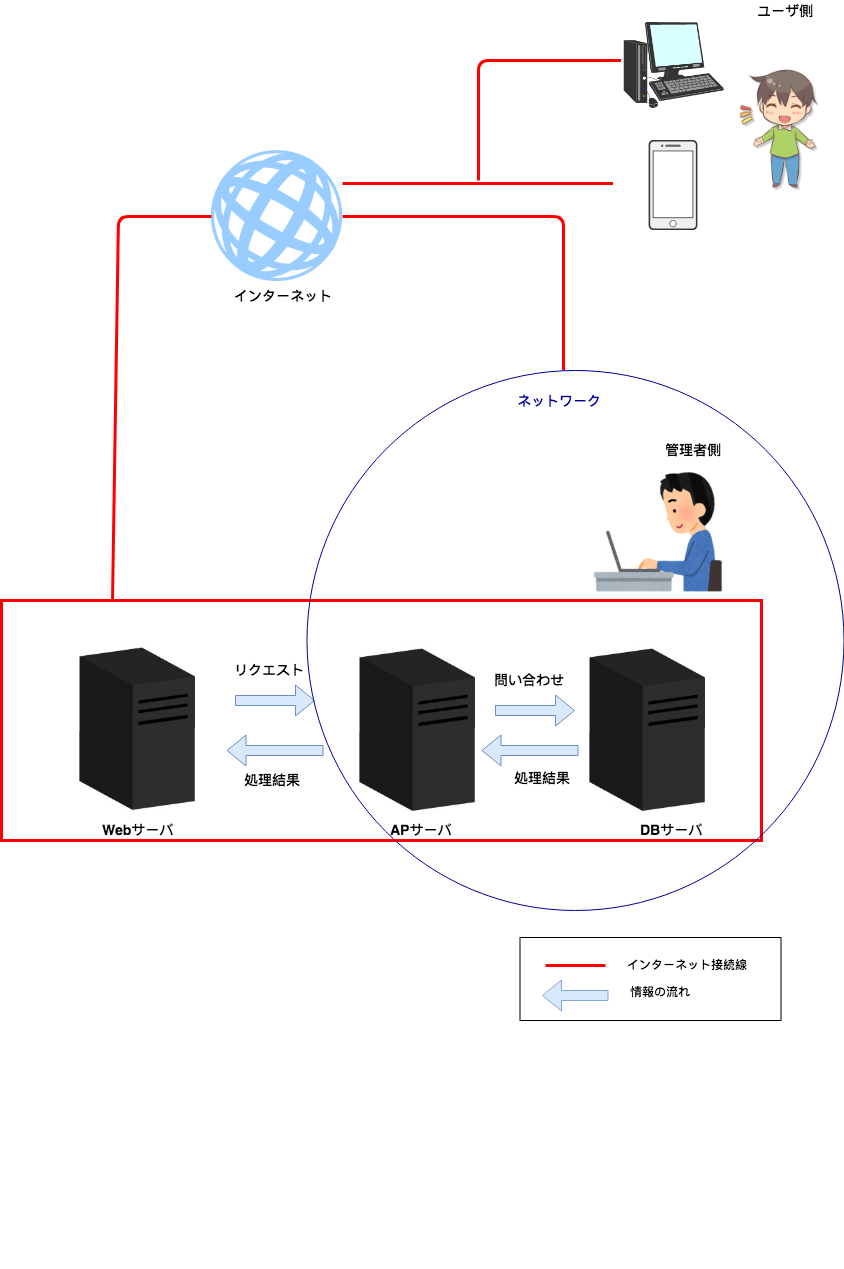
\includegraphics{KUTBBS-network.png}}
\caption{ネットワーク構成}
\label{network:networktest}
\end{center}
\end{figure}




% \bibliographystyle{jplain}
% \begin{thebibliography}{10}
%
%
%
% \end{thebibliography}
\newpage
\appendix
\part*{付録}
\addcontentsline{toc}{part}{付録}

\setcounter{section}{0} % section の番号をゼロにリセットする
\renewcommand{\thesection}{\Alph{section}} % 数字ではなくアルファベットで数える
\setcounter{figure}{0} % 図番号
\renewcommand{\thefigure}{\Alph{section}}


\section{ユースケース図}
図\ref{UseCase:UseCasetest}に、本システムのユースケース図を示す。
\begin{figure}[H]
\begin{center}
\resizebox{10cm}{!}{\includegraphics{UseCase.png}}
\caption{ユースケース図}
\label{UseCase:UseCasetest}
\end{center}
\end{figure}

\newpage
\setcounter{figure}{0} % 図番号
\renewcommand{\thefigure}{\Alph{section}-\arabic{figure}}

\section{KUTBBSの画面遷移図}
\label{Screen_transition}
図\ref{fig:Screen_transition_1}、図\ref{fig:Screen_transition_2}に、本システムの画面遷移図を示す。
\begin{figure}[H]
\centering
\resizebox{16cm}{!}{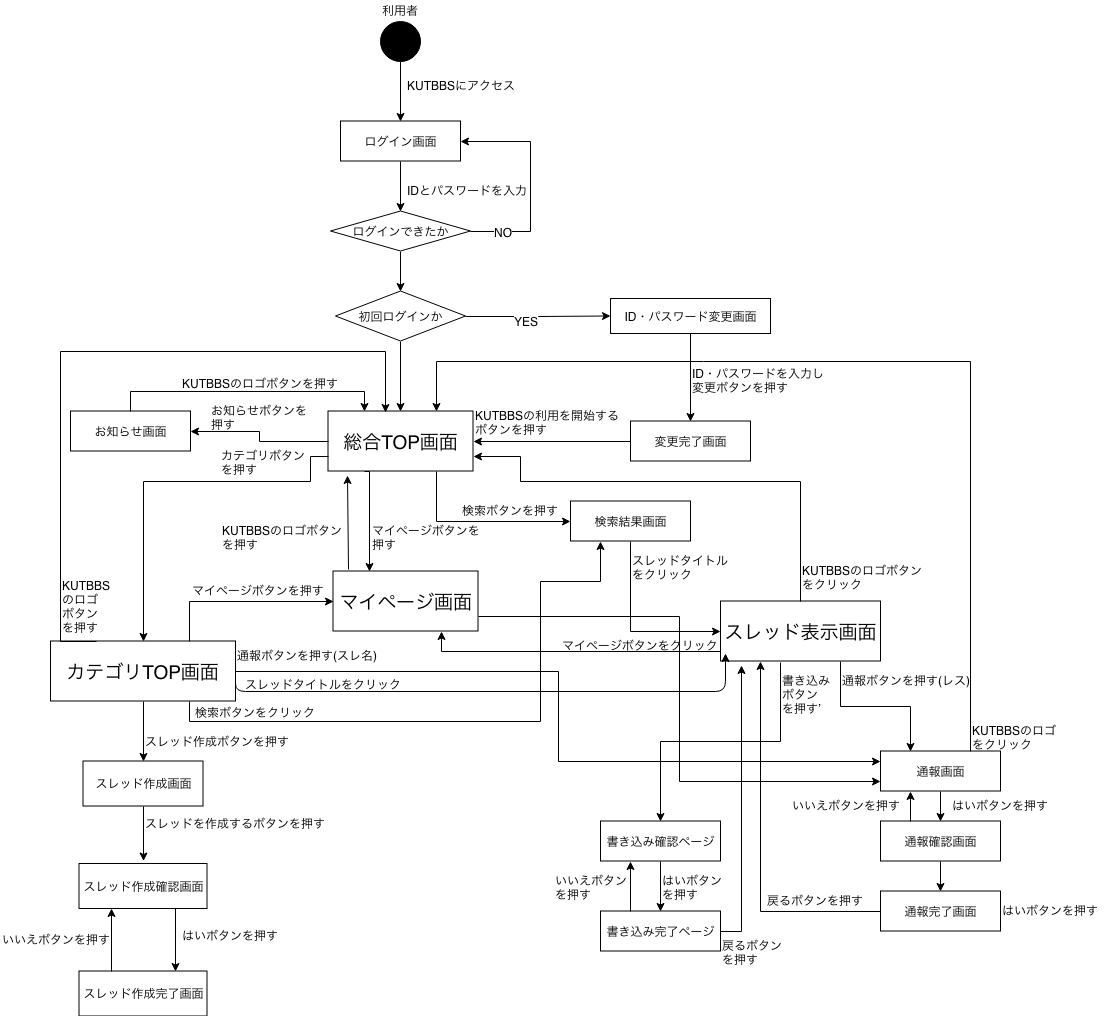
\includegraphics{利用者の画面遷移図.png}}
\caption{学生掲示板KUTBBSの画面遷移図}
\label{fig:Screen_transition_1}
\end{figure}

\begin{figure}[H]
\centering
\resizebox{16cm}{!}{\includegraphics{管理者の画面遷移図.png}}
\caption{管理者側の画面遷移図}
\label{fig:Screen_transition_2}
\end{figure}

\end{document}
